% глава 3

\chapter{Исследование пуско-тормозных режимов работы ленточного конвейера} \label{chapt3}
В~данной главе рассматривается выбор и описание математической модели ленточного конвейера, ее доработки, требуемые для дальнейших исследований, а~также анализ переходных процессов, возникающих при~пуске, изменении скорости и~торможении ленточного конвейера с~одним приводом и~натяжным устройством, расположенном в~хвостовой части. В~частности, в~главе представлен анализ переходных процессов, возникающих при~переключении скорости ленты конвейера, анализ переходных процессов, возникающих при~торможении как~приводного, так и~хвостового барабанов конвейера, анализ переходных процессов, возникающих при~останове (свободном выбеге) конвейера.

Для~исследования выберем подземный ленточный конвейер \textbf{1Л-100К} с~тканевой лентой, предназначенный для~использования в~выработках с~углами наклона от $-3^\circ$ до $+18^\circ$. Приемная способность этого конвейера составляет $11\text{м}^3/\text{мин}$, ширина ленты $1000\text{мм}$, скорость движения ленты $1,6\text{м/с}$, диаметр приводного барабана  $800\text{мм}$, производительность  $420\text{т/час}$. В~соответствии с~графиками применимости \cite{Aevnevich} длина конвейерной установки при угле наклона выработки $0^\circ$  составляет $1000\text{м}$. 
Конвейер имеет однобарабанный привод с~тяговым фактором $e^{\mu\alpha} = 2,5$. Подробные технологические параметры рассматриваемого ленточного конвейера указаны в~таблице~\ref{tabl:konv_params}.

В работе~\cite{vdmitrieva} описано построение математической модели двухбарабанного конвейера.
При~построении модели процессы, происходящие в ленте конвейера, рассматриваются с~точки зрения распространения волн напряжения и~деформаций. Для~решения волнового уравнения при~исследовании переходных режимов конвейера в работе использован известный метод линейно-кусочной аппроксимации, который был предложен для~решения подобной задачи О.А. Залесовым и~использованный И. В. Запениным~\cite{izapenin1}, \cite{izapenin2}. Этот метод позволил достаточно точно описать движение системы с~распределенными параметрами, описываемой дифференциальными уравнениями в~частных производных, системой с~сосредоточенными параметрами, движение которой описывается обыкновенными дифференциальными уравнениями.

При использовании этой математической модели конвейера принимаются следующие допущения:
\begin{itemize}
\item трасса конвейера прямолинейна и~имеет постоянный угол наклона;
\item трансмиссионные валы и~муфты абсолютно жесткие. В~этом случае приводное устройство может быть представлено в~виде одной сосредоточенной массы;
\item масса ленты и~вращающихся частей роликоопор равномерно распределена;
\item проскальзывание ленты на~роликоопорах отсутствует;
\item лента представляется упруго-вязким стержнем;
\item силы внутреннего трения пропорциональны скорости деформации;
\item масса хвостового барабана пренебрежимо мала по~сравнению с~распределенной массой ленты и~груза;
\item коэффициенты сопротивления движению на~грузовой и~порожней ветвях ленты постоянны;
\item скорости ленты в~точках набегания и~сбегания на~приводном барабане равны.
\end{itemize}

\begin{table}[h]
\caption{Параметры магистрального ленточного конвейера 1Л-100К}
\label{tabl:konv_params}
\begin{center}
\begin{tabular}{|l|l|}
\hline
Длина ленты $l$, м & 1000 \\
\hline
Ширина ленты $k$, м & 1 \\
\hline
Скорость движения ленты $v$, м/c & 1,6 - 2,5 \\
\hline
Погонный вес движущихся частей на грузовой ветви $q_\text{г}, \text{Н/м}$ & 1045\\
\hline
Погонный вес движущихся частей на порожней ветви $q_\text{п}, \text{Н/м}$ & 250\\
\hline
Вес груза натяжного устройства $G_\text{ну}, \text{Н}$ & 80000 \\
\hline
Масса участка грузовой ветви $m_\text{г}, \text{кг}$ & 870,8 \\
\hline
Масса участка порожней ветви $m_\text{п}, \text{кг}$ & 208,3 \\
\hline
Масса привода $m_\text{пр}, \text{кг}$ & 1850 \\
\hline
Радиус приводного барабана $R_\text{б}, \text{мм}$ & 400 \\
\hline
Коэффициент сопротивления движению $w$ & 0,03 \\
\hline
Коэффициент сопротивления движению натяжных грузов $f$ & 0,3 \\
\hline
Вязкость ленты с грузом $\eta, \text{Н/м} $ & 1100 \\
\hline
Жесткость ленты $C, \text{Н/м} $ & 1000 \\
\hline
Жесткость канатов натяжного устройства $ C_k, \text{Н/м} $ & $ 5 \times 10^5 $ \\
\hline
\end{tabular}
\end{center}
\end{table}

\section{Математическая модель одноприводного двухбарабанного ленточного конвейера с натяжным устройством, расположенным в хвостовой части} \label{sect3_1}

Расчетная схема для~конвейера с~однобарабанным головным приводом и~натяжным устройством, расположенным в~хвостовой части конвейера, представлена на~рис.~\ref{img:3.sheme}. При~построении математической модели распределенная масса ленты с~грузом представлена тремя массами на~грузовой ветви и~одной массой на~порожней ветви. В~качестве обобщенных переменных приняты координаты положения четырех сосредоточенных масс $m_1, m_2, m_3, m_4$, их~скорости $\dot x_1, \dot x_2, \dot x_3, \dot x_4$, перемещения $x_1, x_2, x_3, x_4$, а~так~же положение и~скорость перемещения натяжного устройства $\delta, \dot \delta$. Конечномерная математическая модель движения конвейера с~грузом \cite{vdmitrieva1}, \cite{vdmitrieva2} описана десятью координатами состояния $X = (x_1, x_2, x_3, x_4, \dot x_1, \dot x_2, \dot x_3, \dot x_4, \delta, \dot \delta)^T$.

\if 0
Уравнения движения для~конвейера представлены системой дифференциальных уравнений, составленных с~использованием метода кусочно-линейной аппроксимации~\cite{izapenin1} по~общей схеме уравнения Лагранжа второго рода:

$$ \frac{d}{dt} \left( \frac{\partial}{\partial \dot x_i} T \right) - \left( \frac{\partial}{\partial x_i} T \right) + \frac{\partial}{\partial x_i} \text{П} + \frac{\partial}{\partial x_i} A = 0, $$

где $ T $ - кинетическая энергия участка, $ \text{П} $ - потенциальная энергия участка, $ A $ - работа внешних сил на~участке.
\\

Кинетическая энергия системы для~рассматриваемой расчетной схемы складывается из~кинетической энергии замкнутого контура ленты с~равномерно распределенным на~ней грузом на~верхней ветви $T_\text{К}$, кинетической энергии $T_\text{П}$ приводного и~натяжного $T_\text{Н}$ устройств:

$$ T_\text{К} = \frac{G_\text{г}l}{6g}(\dot x_1^2 + \dot x_1 \dot x_2 + \dot x_2^2  ) + \frac{G_\text{г}l}{6g}(\dot x_2^2 + \dot x_2 \dot x_3 + \dot x_3^2) + \frac{G_\text{п}l}{6g}(\dot x_1^2 + \dot x_1 \dot x_4 + \dot x_4^2  ) + \frac{G_\text{п}l}{6g}(\dot x_4^2 + \dot x_4 \dot x_3 + \dot x_3^2  ), $$

где $ G_\text{г}, G_\text{п} $ - погонный вес движущихся частей соответственно груженной и~порожней ветвей.

Кинетическая энергия приводного устройства:

$$ T_\text{П} = \frac{m_\text{пр} \dot x_1^2}{2}, $$

где $ m_\text{пр} $ - масса вращающихся частей электродвигателя, редуктора, муфт и~приводного барабана, приведенная к~ободу барабана.

Кинетическая энергия натяжного устройства:

$$ T_\text{Н} = \frac{G_\text{ну} \dot \delta^2}{2g}, $$

где $ G_\text{ну}, \dot \delta $ - соответственно вес и~скорость перемещения натяжного устройства.

Суммируя полученные выражения и~производя алгебраические преобразования, получим выражения для~полной кинетической энергии системы:

 \begin{eqnarray} T_\Sigma = \frac{G_\text{г}l}{6g}(\dot x_1^2 + \dot x_1 \dot x_2 + \dot x_2^2  ) + \frac{G_\text{г}l}{6g}(\dot x_2^2 + \dot x_2 \dot x_3 + \dot x_3^2) + \frac{G_\text{п}l}{6g}(\dot x_1^2 + \dot x_1 \dot x_4 + \dot x_4^2  ) + \nonumber \\ + \frac{G_\text{п}l}{6g}(\dot x_4^2 + \dot x_4 \dot x_3 + \dot x_3^2  ) + \frac{m_\text{пр} \dot x_1^2}{2} + \frac{G_\text{ну} \dot \delta^2}{2g}, \nonumber \end{eqnarray} 

Найдя производные по~времени от~частных производных кинетической энергии для~каждой обобщенной координаты, получим:

$$ \frac{d}{dt} \Big(\frac{\partial}{\partial \dot x_1}T_\Sigma \Big) = \frac{G_\text{г}l}{6g}(2 \ddot x_1 + \ddot x_2 ) +  \frac{G_\text{п}l}{6g}(2 \ddot x_1 + \ddot x_4 ) + m_\text{пр} \ddot x_1, $$


$$ \frac{d}{dt} \Big(\frac{\partial}{\partial \dot x_2}T_\Sigma \Big) = \frac{G_\text{г}l}{6g}(2 \ddot x_2 + \ddot x_3 ) +  \frac{G_\text{г}l}{6g}(2 \ddot x_2 + \ddot x_1 ), $$

$$ \frac{d}{dt} \Big(\frac{\partial}{\partial \dot x_3}T_\Sigma \Big) = \frac{G_\text{г}l}{6g}(2 \ddot x_3 + \ddot x_2 ) +  \frac{G_\text{п}l}{6g}(2 \ddot x_3 + \ddot x_4 ), $$

$$ \frac{d}{dt} \Big(\frac{\partial}{\partial \dot x_4}T_\Sigma \Big) = \frac{G_\text{п}l}{6g}(2 \ddot x_4 + \ddot x_3 ) +  \frac{G_\text{п}l}{6g}(2 \ddot x_4 + \ddot x_1 ), $$

$$ \frac{d}{dt} \Big(\frac{\partial}{\partial \delta}T_\Sigma \Big) = \frac{G_\text{ну}}{g} \ddot \delta. $$\\

Потенциальная энергия упругой деформации системы при~принятых допущениях состоит из~энергии замкнутого контура $ \text{П}_\text{К} $ конвейерной ленты и~канатов натяжного устройства $ \text{П}_\text{Н} $.

$$ \text{П}_\text{К} = \frac{(x_1 - x_2)^2 C_1}{2} + \frac{(x_2 - x_3)^2 C_2}{2} + \frac{(x_4 - x_1)^2 C'_1}{2} + \frac{(x_3 - x_4)^2 C'_2}{2}, $$

где $ C_1, C_2, C'_1, C'_2 $ – коэффициенты жесткости соответствующих участков конвейерной ленты. Так~как участки ленты однородны, то~предполагаются равными их~коэффициенты жесткости, следовательно:

$$ \text{П}_\text{К} = \frac{(x_1 - x_2)^2 C}{2} + \frac{(x_2 - x_3)^2 C}{2} + \frac{(x_4 - x_1)^2 C}{2} + \frac{(x_3 - x_4)^2 C}{2}, $$

где $ C $ – коэффициент жесткости каждого участка.

Потенциальная энергия канатов натяжного устройства:

$$ \text{П}_\text{Н} = 0,5 \Big( \frac{x_3 - x_4}{2} - \delta \Big)^2 C_K, $$

где $ C_K $ – коэффициент жесткости каната, $ \delta $ - перемещение натяжного устройства.

Потенциальная энергия положения натяжного груза:

$$ \text{П}_\text{г} = G_\text{ну} \delta. $$

Найдем частные производные по~обобщенным координатам от потенциальной энергии:

$$ \frac{\partial}{\partial x_1}\text{П} = \Big( \frac{2x_1 - 2x_2}{2} \Big) C + \Big( \frac{2x_1 - 2x_4}{2} \Big)C = (x_1 - x_2)C + (x_1 - x_4)C;$$

$$ \frac{\partial}{\partial x_2}\text{П} = \Big( \frac{2x_2 - 2x_1}{2} \Big) C + \Big( \frac{2x_2 - 2x_3}{2} \Big)C = (x_2 - x_1)C + (x_2 - x_3)C;$$

\begin{eqnarray} 
\frac{\partial}{\partial x_3}\text{П} = 	\Big( \frac{2x_3 - 2x_2}{2} \Big) C + 
		  				\Big( \frac{2x_3 - 2x_4}{2} \Big)C + 
						\frac{x_3 - x_4}{4}C_K + 
						\frac{\delta}{2}C_K = 
					\nonumber \\ = 
						(x_3 - x_2)C + 
						(x_3 - x_4)C + 
						x_3 0.25 C_K - 
						x_4 0.25 C_K - 
						\delta 0.5 C_K;  
					\nonumber 
\end{eqnarray}

 \begin{eqnarray} \frac{\partial}{\partial x_4}\text{П} = \Big( \frac{2x_4 - 2x_3}{2} \Big) C + \Big( \frac{2x_4 - 2x_1}{2} \Big)C + \frac{x_4 - x_3}{4}C_K + \frac{\delta}{2}C_K = \nonumber \\ = (x_4 - x_3)C + (x_4 - x_1)C + x_4 0.25 C_K - x_3 0.25 C_K + \delta 0.5 C_K;  \nonumber \end{eqnarray}

$$ \frac{\partial}{\partial \delta}\text{П} = -x_3 0.5 C_K + x_4 0.5 C_K + \delta C_K - G_{\text{ну}}$$\\

Работа внешних сил складывается из~работы движущей силы привода, сил сопротивления движению ветвей ленты и~натяжных грузов, а~также силы торможения.

Работа движущей силы привода:

$$ A_{\text{пр}} = - \frac{ M_{\text{пр}} }{ R_{\text{б}} } x_1, $$

Где $ M_{\text{пр}} $ – момент двигателя, приведенный к~валу приводного барабана, $x_1$ - управляющее воздействие, $ R_{\text{б}} $ – радиус приводного барабана.

Работа сил сопротивления движению ветвей ленты:

$$ A_K = G_{\text{г}} l w' \frac{x_1 + x_2}{2}  + 
                G_{\text{г}} l w' \frac{x_1 + x_3}{2}  + 
                G_{\text{п}} l w'' \frac{x_1 + x_4}{2} + 
                G_{\text{п}} l w'' \frac{x_4 + x_3}{2}, 
$$

где  $ w' $ и $ w'' $, – коэффициенты сопротивления движению груженой и~порожней ветвей. В~дальнейшем их~примем равными. Силы сопротивления движению участков $ W_i $  всегда направлены противоположно скорости $ \dot x_i $ этих участков, то~есть $ W_i = G_i l_ij w \text{sgn} \dot x_i $.

Работа сил сопротивления движению натяжных грузов:

$$ A_{\text{н}} = \pm G_{\text{ну}} f \delta , $$

где $ f $ - приведенный коэффициент сопротивления движению натяжных грузов.\\

Найдены частные производные по~обобщенным координатам работы сил сопротивления движению:

$$ \frac{ \partial }{ \partial x_1} A = - \frac{ M_{\text{пр}} }{ R_{\text{б}} } \text{sgn} ( \dot x_c - \dot x_1 ) + 0.5 G_{\text{г}} l w \text{sgn} \dot x_1 +  0.5 G_{\text{п}} l w \text{sgn} \dot x_1, $$

$$ \frac{ \partial }{ \partial x_2} A = 0.5 G_{\text{г}} l w \text{sgn} \dot x_2 + 0.5 G_{\text{г}} l w \text{sgn} \dot x_2 = G_{\text{г}} l w \text{sgn} \dot x_2, $$

$$ \frac{ \partial }{ \partial x_3} A = 0.5 G_{\text{г}} l w \text{sgn} \dot x_3 + 0.5 G_{\text{п}} l w \text{sgn} \dot x_3, $$

$$ \frac{ \partial }{ \partial x_4} A = 0.5 G_{\text{п}} l w \text{sgn} \dot x_4 + 0.5 G_{\text{п}} l w \text{sgn} \dot x_4 = G_{\text{п}} l w \text{sgn} \dot x_4, $$

$$ \frac{ \partial }{ \partial \delta } A =  G_{\text{п}} f апт \dot \delta . $$

Работа сил внутреннего трения замкнутого контура:

$$ A_{\text{в}} = 	(\dot x_1 - \dot x_2)(x_1 - x_2) \eta + 
			(\dot x_2 - \dot x_3)(x_2 - x_3) \eta + 
			(\dot x_3 - \dot x_4)(x_3 - x_4) \eta + 
			(\dot x_4 - \dot x_1)(x_4 - x_1) \eta, $$

где $ \eta $  – приведенный коэффициент вязкости.

Частные производные по~координатам от~работы сил внутреннего трения:

$$ \frac{ \partial }{ \partial x_1} A_{\text{в}} = (\dot x_1 - \dot x_2) \eta + (\dot x_1 - \dot x_4) \eta, $$

$$ \frac{ \partial }{ \partial x_2} A_{\text{в}} = (\dot x_2 - \dot x_3) \eta + (\dot x_2 - \dot x_3) \eta, $$

$$ \frac{ \partial }{ \partial x_3} A_{\text{в}} = (\dot x_3 - \dot x_4) \eta + (\dot x_3 - \dot x_2) \eta, $$

$$ \frac{ \partial }{ \partial x_4} A_{\text{в}} = (\dot x_4 - \dot x_1) \eta + (\dot x_4 - \dot x_3) \eta, $$

$$ \frac{ \partial }{ \partial \delta} A_{\text{в}} = 0 . $$\\

Систему дифференциальных уравнений получим, суммируя производные по~времени от~частных производных кинетической энергии по~обобщенным координатам с~частными производными по~обобщенным координатам от~потенциальной энергии деформации ленты, работы сил сопротивления движению, сил внутреннего трения и~работы движущей силы привода.

Введя обозначения $ \frac{ G_{\text{г}} l }{6g} = m_{\text{г}} $, $ \frac{ G_{\text{п}} l }{6g} = m_{\text{п}} $, получим математическую модель конвейера, представляющую собой систему из~пяти нелинейных дифференциальных уравнений второго порядка: 

\begin{eqnarray}
	m_{\text{г}} (2 \ddot x_1 + \ddot x_2 ) +  m_{\text{п}} (2 \ddot x_1 + \ddot x_4 ) + m_{\text{пр}} \ddot x_1 + (2x_1 - x_2 - x_4)C + 0.5(G_{\text{г}} + G_{\text{п}}) l w \text{sgn} \dot x_1 +
\nonumber \\
	+ (2 \dot x_1 - \dot x_2 - \dot x_4) \eta = \frac{M_{\text{пр}}}{R_{\text{б}}} \text{sgn} (\dot x_c - \dot x_1),
\nonumber
\end{eqnarray}

\begin{eqnarray}
	m_{\text{г}} (2 \ddot x_2 + \ddot x_3 ) + m_{\text{г}} (2 \ddot x_2 + \ddot x_1 ) + (2x_2 - x_1 - x_3)C +  G_{\text{г}} l w \text{sgn} \dot x_2 +  (2 \dot x_2 - \dot x_1 - \dot x_3) \eta = 0,
\nonumber
\end{eqnarray}

\begin{eqnarray}
	m_{\text{г}} (2 \ddot x_3 + \ddot x_2 ) + m_{\text{п}} (2 \ddot x_3 + \ddot x_4 ) + (2x_3 - x_2 - x_4)C + 0,25 (x_3 - x_4 - 2 \delta) C_K +
\nonumber \\
	+ (2 \dot x_3 - \dot x_2 - \dot x_4) \eta + 0.5 ( G_{\text{г}} + G_{\text{п}} ) l w \text{sgn} \dot x_3 = 0,
\nonumber
\end{eqnarray}

\begin{eqnarray}
	m_{\text{п}} (2 \ddot x_4 + \ddot x_3 ) + m_{\text{п}} (2 \ddot x_4 + \ddot x_1 ) + (2x_4 - x_1 - x_3)C + 0,25 (x_4 - x_3 + 2 \delta) C_K +
\nonumber \\
	+  G_{\text{п}}) l w \text{sgn} \dot x_4 +  (2 \dot x_4 - \dot x_1 - \dot x_3) \eta = 0,
\nonumber
\end{eqnarray}

\begin{eqnarray}
	\frac{G_{\text{ну}}}{g} \ddot \delta - 0,5(x_4 - x_3 + \delta)C_K + G_{\text{ну}} + G_{\text{ну}} f \text{sgn} \dot \delta = 0.
\nonumber
\end{eqnarray}
\fi

Подробный расчет модели приведен в работе~\cite{vdmitrieva1}. Ниже приведена результирующая система дифференциальных уравнений, описывающих совместное движение равномерно загруженной ленты конвейера:
\clearpage

\begin{figure} [h] 
  \center
  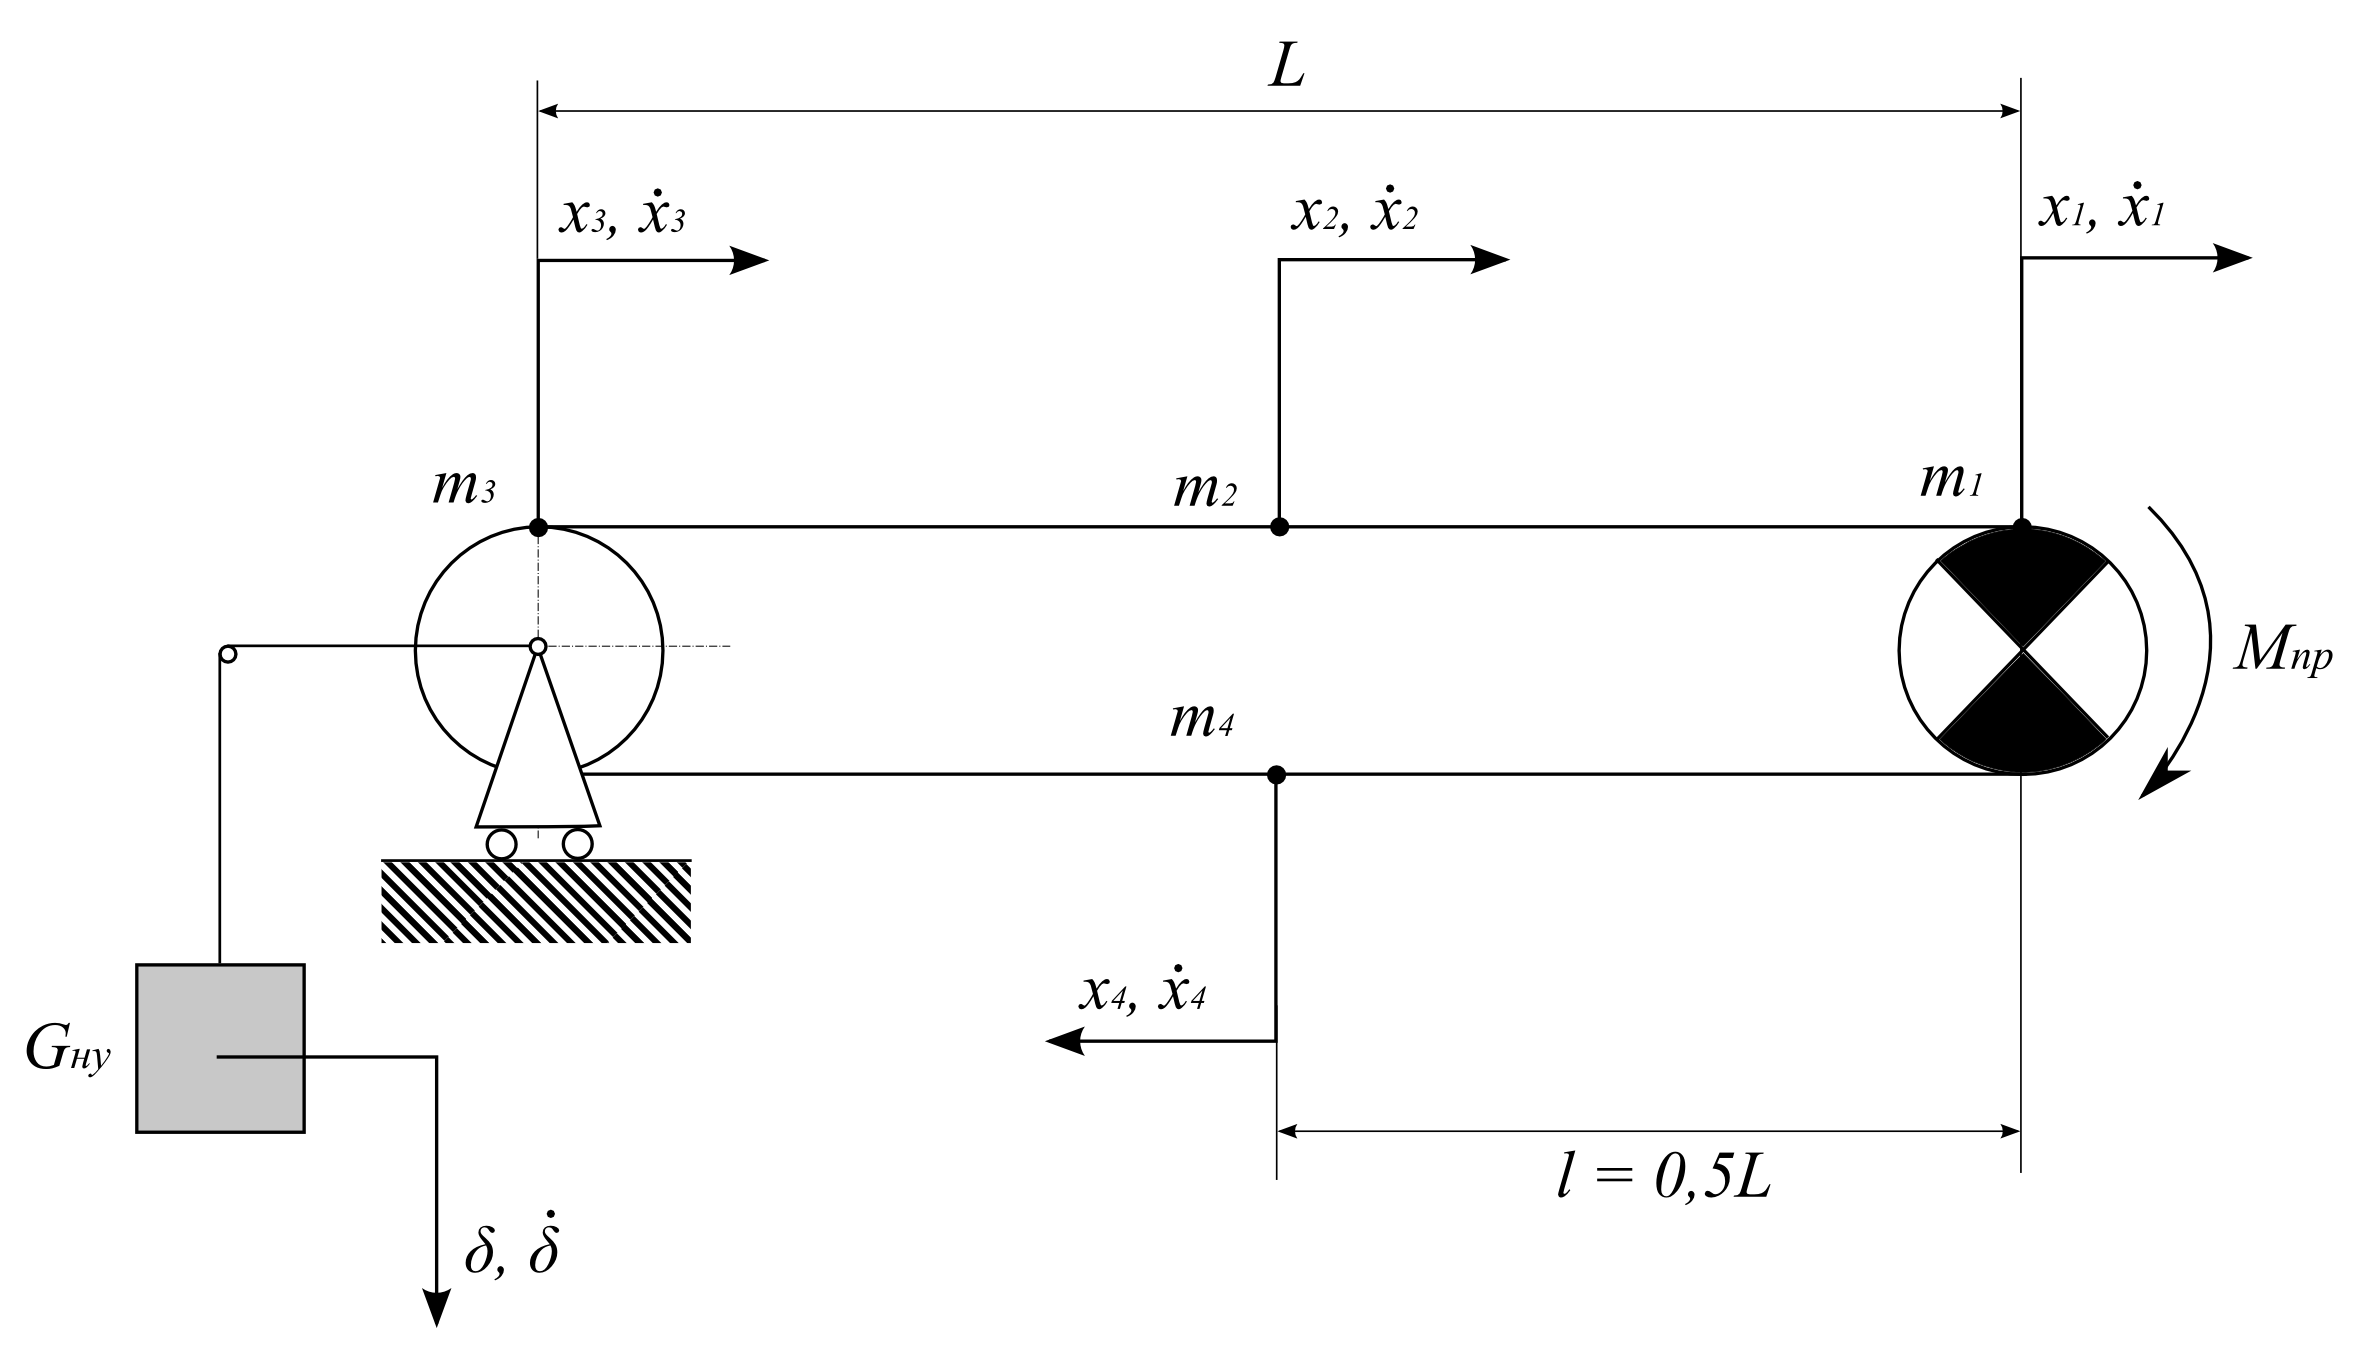
\includegraphics [scale=0.25] {3-1-0}
  \caption{Расчетная схема конвейера с натяжным устройством, расположенным в хвостовой части конвейера.} 
  \label{img:3.sheme}  
\end{figure}

\begin{eqnarray}
	( 2m_{\text{г}} + 2m_{\text{п}} + m_{\text{пр}} ) \ddot x_1 +  m_{\text{г}} \ddot x_2 +  m_{\text{п}} \ddot x_4  + 2Cx_1 - Cx_2 - Cx_4 + (0.5 G_{\text{п}} l w + 0.5 G_{\text{г}} l w ) \text{sgn} \dot x_1 +
\nonumber \\
	+ 2 \eta \dot x_1 - \eta \dot x_2 - \eta \dot x_4 = \frac{M_{\text{пр}}}{R_{\text{б}}} \text{sgn} (\dot x_c - \dot x_1),
\nonumber
\end{eqnarray}

\begin{eqnarray}
	m_{\text{г}} \ddot x_1 + 4 m_{\text{г}} \ddot x_2 + m_{\text{г}} \ddot x_3 - Cx_1 + 2Cx_2 - Cx_3 + G_{\text{г}}) l w \text{sgn} \dot x_2  - \eta \dot x_1 + 2 \eta \dot x_2 - \eta \dot x_3 = 0,
\nonumber
\end{eqnarray}

\begin{eqnarray}
	m_{\text{г}} \ddot x_2 + ( 2 m_{\text{г}} + m_{\text{п}} ) \ddot x_3 + m_{\text{п}} \ddot x_4  - Cx_2  + (2C + 0,25C_K) x_3 - (C + 0,25 C_K) x_4 - 
\nonumber \\
	- 0,5C_K \delta - \eta \dot x_2 + 2 \eta \dot x_3 - \eta \dot x_4 + (0.5 G_{\text{г}} l w + 0,5 G_{\text{п}} ) l w) \text{sgn} \dot x_3 = 0,
\nonumber
\end{eqnarray}

\begin{eqnarray}
	m_{\text{п}} \ddot x_1 + m_{\text{п}} \ddot x_3 + 4 m_{\text{п}} \ddot x_4 - Cx_1 - (2C + 0,25 C_K) x_3 + (C + 0,25 C_K) x_4  + 0,5 C_K \delta -
\nonumber \\
	- \eta \dot x_1 - \eta \dot x_3 + 2 \eta \dot x_4 G_{\text{п}}) l w \text{sgn} \dot x_4 = 0,
\nonumber
\end{eqnarray}

\begin{eqnarray}
	\frac{G_{\text{ну}}}{g} \ddot \delta - 0,5 C_K x_3 + 0,5 C_K x_4 + C_K \delta + G_{\text{ну}} + G_{\text{ну}} f \text{sgn} \dot \delta = 0,
\nonumber
\end{eqnarray}

где $ m_{\text{г}} = \frac{G_{\text{г}} l }{6g}, $ $ m_{\text{п}} = \frac{G_{\text{п}} l}{6g} $, $ G_{\text{г}} $ -- погонный вес грузовой ветви, $ G_{\text{п}} $ -- погонный вес порожней ветви, $ l = 0,5L $, $ L $ -- длина конвейера. $ C $ -- коэффициент жесткости ленты, $ w $ -- коэффициент сопротивления движению ленты, $ \eta $ -- приведенный коэффициент вязкости ленты, $ C_K $ -- коэффициент жесткости каната натяжного устройства, $ G_{\text{ну}} $ -- вес натяжного устройства, $ f $ -- приведенный коэффициент сопротивления движению натяжных грузов, $ M_{\text{пр}} $ -- момент двигателя, приведенный к~валу приводного барабана, $ R_{\text{б}} $ -- радиус барабана.

Для~лаконичного представления системы уравнений она записана в~матричном виде относительно вектора состояния  $ X = (x_1, x_2, x_3, x_4, \delta)^T $:

$$ M \ddot X + N \dot X + CX + S \text{sgn} \dot X + G = P \text{sgn} ( \dot X_c - \dot X_1 ) M_{\text{пр}}, $$

где:

$$ 
M = 
\begin{bmatrix}
	2m_{\text{г}} + 2m_{\text{п}} + m_{\text{пр}} & m_{\text{г}} & 0              & m_{\text{п}}                    & 0                                 \\
	m_{\text{г}}                                                 & 4 m_{\text{г}} & m_{\text{г}}                    & 0              & 0                \\
	0                                                            & m_{\text{г}}   & 2 m_{\text{г}} + 2 m_{\text{п}} & m_{\text{п}}   & 0 \\
	m_{\text{п}}                                                 & 0              & m_{\text{п}}                    & 4 m_{\text{п}} & 0   \\
	0                                                            & 0              & 0                               & 0              & G_{\text{ну}} g^{-1}
\end{bmatrix},
$$

$$
N = 
\begin{bmatrix}
	2 \eta & - \eta & 0      & - \eta & 0 \\
	- \eta & 2 \eta & - \eta & 0      & 0 \\
	0      & - \eta & 2 \eta & - \eta & 0 \\
	- \eta & 0      & - \eta & 2 \eta & 0 \\
	0      & 0      & 0      & 0      & 0
\end{bmatrix}, P = 
\begin{bmatrix}
	R_{\text{б}}^{-1} \\
	0                 \\
	0                 \\
	0                 \\
	0
\end{bmatrix}, G = 
\begin{bmatrix}
	0                 \\
	0                 \\
	0                 \\
	0                 \\
	G_{\text{ну}}
\end{bmatrix},
$$

$$ S = diag [ 0,5 G_{\text{г}} l w + 0,5 G_{\text{п}} l w \quad G_{\text{г}} l w \quad 0,5 G_{\text{г}} l w + 0,5 G_{\text{п}} l w \quad G_{\text{п}} l w \quad G_{\text{ну}} f], $$

$$ 
C = 
\begin{bmatrix}
	2C & -C & 0             & -C            & 0         \\
	-C & 2C & -C            & 0             & 0         \\
	0  & -C & 2C + 0,25C_K  & -C - 0,25 C_K & -0,5 C_K  \\
	-C & 0  & -C - 0,25 C_K & 2C + 0,25C_K  & 0,5 C_K   \\
	0  & 0  & -0,5 C_K      & 0,5 C_K       & C_K
\end{bmatrix}.
$$

Для~получения канонического представления этой модели все~члены уравнения умножены на~матрицу $ M^{-1} $:

$$ \ddot X + M^{-1} N \dot X + M^{-1} C X + M^{-1} S \text{sgn} \dot X + M^{-1} G = M^{-1} P \text{sgn} ( \dot X_c - \dot X_1 ) M_{\text{пр}}. $$

\if 0
Далее рассчитаем суммарный погонный вес движущихся частей на~грузовой ветви: 

$$ q_{\text{ гр} \Sigma} = q_{\text{л}} + q'_{\text{р}} + q_{\text{гр}}, $$

где $ q_{\text{л}} $ – погонный вес ленты, Н/м, $ q'_{\text{р}} $  – погонный вес роликов, Н/м, $ q_{\text{гр}} $ – погонный вес груза, Н/м.

Рассчитаем погонный вес груза: 

$$ q_{\text{гр}} = \frac{Q}{0,36 v}, $$

где $Q$ - эксплуатационная производительность конвейера, т/ч , $v$ – номинальная скорость движения ленты, м/с.

$$ q_{\text{гр}} = \frac{420}{0,36 \times 1,6} = 695 \text{Н/м}. $$

Рассчитаем $ q'_p $, погонный вес вращающихся частей роликов грузовой ветви по~формуле: 

$$ q'_p = \frac{G'_p}{l'_p}, $$

где $ G'_p $ - вес вращающихся частей роликов на~грузовой ветви, $ G'_p = 215 \text{Н} $, $ l'_p $ – расстояние между роликоопорами на~грузовой ветви, $ l'_p = 1,1 \text{м}. $

$$ q'_p = \frac{215}{1,1} = 195 \text{Н/м}. $$

Погонный вес ленты принимаем равным 150 Н/м.

Суммарный погонный вес движущихся частей на~грузовой ветви составляет

$$ q_{\text{ гр} \Sigma} = q_{\text{л}} + q'_{\text{р}} + q_{\text{гр}} = 1040 \text{Н/м}. $$

Рассчитаем $ q_{\text{п} \Sigma} $ - суммарный погонный вес движущихся частей порожней ветви:

$$ q_{\text{п} \Sigma} = q_{\text{л}} + q''_{\text{р}}, $$

где $ q''_p $ - погонный вес роликов на~порожней ветви, $ q_{\text{л}} $ - погонный вес ленты.

Погонный вес роликов на~порожней ветви: 

$$ q''_p = \frac{G''_p}{l''_p}, $$

где $ G''_p $ - вес вращающихся частей роликов на~порожней ветви, $ G''_p = 220 \text{Н} $, $ l''_p $ – расстояние между роликоопорами на~порожней ветви, $ l''_p = 2,2 \text{м}. $

$$ q''_p = \frac{220}{2,2} = 100 \text{Н/м}. $$

Суммарный погонный вес движущихся частей на~порожней ветви:

$$ q_{\text{п} \Sigma} = q_{\text{л}} + q''_{\text{р}} = 150 + 100 = 250 \text{Н/м}. $$

Матрицы M,~N,~C,~S систем уравнений математической модели принимают вид:

$$ 
M = 
\begin{bmatrix}
	4008,2 & 870,9  & 0      & 208,3 & 0    \\
	807,8  & 3483,2 & 870,8  & 0     & 0    \\
	0      & 870,8  & 2158,2 & 208,3 & 0    \\
	208,3  & 0      & 208,3  & 833,2 & 0    \\
	0      & 0      & 0      & 0     & 3000
\end{bmatrix},
$$

$$
N = 
\begin{bmatrix}
	2200  & -1100 & 0     & -1100 & 0       \\
	-1100 & 2200  & -1100 & 0     & 0       \\
	0     & -1100 & 2200  & -1100 & 0       \\
	-1100 & 0     & -1100 & 2200  & 0       \\
	0     & 0     & 0     & 0     & 0
\end{bmatrix},
$$

$$ 
C = 
\begin{bmatrix}
	2000  & -1000 & 0       & -1000   & 0       \\
	-1000 & 2000  & -1000   & 0       & 0       \\
	0     & -1000 & 127000  & -126000 & -250000 \\
	-1000 & 0     & -126000 & 127000  & 250000  \\
	0     & 0     & -250000 &  250000 & 500000
\end{bmatrix},
$$

$$
 P = 
\begin{bmatrix}
	2                                \\
	0                                \\
	0                                \\
	0                                \\
	0
\end{bmatrix}, G = 
\begin{bmatrix}
	0                                \\
	0                                \\
	0                                \\
	0                                \\
	30000
\end{bmatrix},
$$

$$ S = diag [ 971,2 \quad 1567,5 \quad 971,2 \quad 375 \quad 2235]. $$
\fi

Числовые значения матриц $ M, N, C, P, G $ приведены в приложении \ref{Appendix11}.\\

Координаты состояния $X = (x_1, x_2, ..., x_10)^T$ введены по каноническому правилу О.~Коши:

$$ 
\begin{matrix}
x_1 = x_1,    & \dot x_1 = x_6,      \\
x_2 = x_2,    & \dot x_2 = x_7,      \\
x_3 = x_3,    & \dot x_3 = x_8,      \\
x_4 = x_4,    & \dot x_4 = x_9,      \\
x_5 = \delta, & \dot x_5 = \dot \delta.
\end{matrix}
$$

В этом случае модель движения ленты конвейера в~пространстве состояний будет представлена в~виде системы нелинейных дифференциальных уравнений:

$$ \dot X =  \tilde{A} X + \tilde{B_1}U_1 + \tilde{B_2} U_2 + \tilde{B_3} U_3, $$

где $ U_1 = M_{\text{пр}} $ -- момент, создаваемый приводом (первое управляющее воздействие), $ U_2 = \text{sgn}X $ -- силы сопротивления движению сосредоточенных масс ленты (второе управляющее воздействие), $ U_3 = G_{\text{ну}} $ -- вес натяжного устройства (третье управляющее воздействие).
$ \tilde{A} $ -- матрица состояний системы, представляет собой блочную матрицу, включающую в~себя матрицы $ M^{-1} N $ и~$ M^{-1} C $ ,  $ \tilde{B_1}, \tilde{B_2}, \tilde{B_3} $ -- матрицы управления. Матрица $ \tilde{B_1} $ включает в~себя $ M^{-1} P $, $\tilde{B_2}$ включает в~себя $ M^{-1} S $, $ \tilde{B_3} $ включает в~себя $ M^{-1} G $:

\if 0
$$
\tilde{A}_{10\times10} = 
\begin{bmatrix}
 0_{5\times5}       & E_{5 \times 5}      \\
 M^{-1}C_{5\times5} & M^{-1}N_{5\times5}  \\
\end{bmatrix},
\tilde{B_1}_{10\times1} = 
\begin{bmatrix}
 0_{5\times1}                             \\
 M^{-1}P_{5\times1}                       \\
\end{bmatrix},
$$

$$
\tilde{B_2}_{10\times10} = 
\begin{bmatrix}
 0_{5\times5} & 0_{5\times5}              \\
 0_{5\times5} & M^{-1}S_{5\times5}        \\
\end{bmatrix},
\tilde{B_3}_{10\times1} = 
\begin{bmatrix}
 0_{5\times1}                             \\
 M^{-1}G_{5\times1}                       \\
\end{bmatrix}.
$$
\fi 

Числовые значения матриц $ \tilde{A}, \tilde{B_1}, \tilde{B_2}, \tilde{B_3} $ приведены приложении \ref{Appendix12}.

\section{Модификация исходной модели конвейера для возможности управления натяжным устройством} \label{sect3_2}
Натяжные устройства сообщают ленте конвейера характерное натяжение, которого хватает для организации передачи на устройстве тяговой силы трением при стабильном движении и~запуске самого конвейера, они ограничивают провисание ленты между роликоопорами, компенсируют удлинение ленты в результате ее вытягивания в процессе работы и сохраняют некоторый запас ленты, необходимый для ее перестановки при повреждениях. В настоящее время натяжные механизмы подразделяются на механические, пневматические, гидравлические, а также грузовые. Модель конвейера, описанная в разделе~\ref{sect3_1}, не позволяет осуществлять управление натяжным устройством.

Под управлением натяжным устройством понимается изменение его веса либо положения каретки для компенсации изменения натяжений грузовой и порожней ветвей. Для того чтобы иметь возможность изменять эти параметры, разделим полученную модель конвейера на две связанных между собой модели – модель, описывающую движение ленты, и модель, описывающую движение натяжного устройства.

\subsection{Модель движения ленты} \label{sect3_2_1}
В модели движения ленты переменными являются перемещения $ x_1, x_2, x_3, x_4 $, скорости $ \dot x_1, \dot x_2, \dot x_3, \dot x_4 $ и ускорения $ \ddot x_1, \ddot x_2, \ddot x_3, \ddot x_4 $ четырех сосредоточенных масс. Положение и скорость натяжного устройства $ \delta $ и $ \dot \delta $ считаются внешними воздействиями $ U_1 $ и $ U_2 $:

\begin{eqnarray}
	( 2m_{\text{г}} + 2m_{\text{п}} + m_{\text{пр}} ) \ddot x_1 +  
	m_{\text{г}} \ddot x_2 +  m_{\text{п}} \ddot x_4  + 
	2Cx_1 - Cx_2 - Cx_4 + 
	(0.5 G_{\text{п}} l w + 0.5 G_{\text{г}} l w ) \text{sgn} \dot x_1 +
    \nonumber \\
	+ 2 \eta \dot x_1 - \eta \dot x_2 - \eta \dot x_4 = 
	\frac{M_{\text{пр}}}{R_{\text{б}}} \text{sgn} (\dot x_c - \dot x_1),
\nonumber
\end{eqnarray}

\begin{eqnarray}
	m_{\text{г}} \ddot x_1 + 4 m_{\text{г}} \ddot x_2 +
	m_{\text{г}} \ddot x_3 - Cx_1 + 2Cx_2 - Cx_3 + 
	G_{\text{г}}) l w \text{sgn} \dot x_2  - 
	\eta \dot x_1 + 2 \eta \dot x_2 - \eta \dot x_3 = 0,
\nonumber
\end{eqnarray}

\begin{eqnarray}
	m_{\text{г}} \ddot x_2 + ( 2 m_{\text{г}} + m_{\text{п}} ) \ddot x_3 + 
	m_{\text{п}} \ddot x_4  - Cx_2 + (2C + 0,25C_K) x_3 - 
   (C + 0,25 C_K) x_4 - 
   \nonumber \\
   - 0,5C_K U_1 - \eta \dot x_2 + 2 \eta \dot x_3 - \eta \dot x_4 + 
   (0.5 G_{\text{г}} l w + 0,5 G_{\text{п}} ) l w) \text{sgn} \dot x_3 = 0,
\nonumber
\end{eqnarray}

\begin{eqnarray}
	m_{\text{п}} \ddot x_1 + m_{\text{п}} \ddot x_3 + 
	4 m_{\text{п}} \ddot x_4 - Cx_1 - 
    (2C + 0,25 C_K) x_3 + (C + 0,25 C_K) x_4 + 
    0,5 C_K U_1 -
    \nonumber \\
	- \eta \dot x_1 - \eta \dot x_3 + 2 \eta \dot x_4 G_{\text{п}}) l w \text{sgn} \dot x_4 = 0,
\nonumber
\end{eqnarray}

В матричном виде система уравнений имеет следующий вид:

$$ M \ddot X + N \dot X + CX + S \text{sgn} \dot X + B_1U_1 = P \text{sgn} ( \dot X_c - \dot X_1 ) M_{\text{пр}}, $$

где:

$ 
M = 
\begin{bmatrix}
	2m_{\text{г}} + 2m_{\text{п}} + m_{\text{пр}} & m_{\text{г}}   & 0                               & m_{\text{п}}   \\
	m_{\text{г}}                                  & 4 m_{\text{г}} & m_{\text{г}}                    & 0              \\
	0                                             & m_{\text{г}}   & 2 m_{\text{г}} + 2 m_{\text{п}} & m_{\text{п}}   \\
	m_{\text{п}}                                  & 0              & m_{\text{п}}                    & 4 m_{\text{п}} 
\end{bmatrix},
$
\bigskip

$
N = 
\begin{bmatrix}
	2 \eta & - \eta & 0      & - \eta \\
	- \eta & 2 \eta & - \eta & 0      \\
	0      & - \eta & 2 \eta & - \eta \\
	- \eta & 0      & - \eta & 2 \eta                                   
\end{bmatrix}, P = 
\begin{bmatrix}
	R_{\text{б}}^{-1}                 \\
	0                                 \\
	0                                 \\
	0                      
\end{bmatrix}, B = 
\begin{bmatrix}
	0                                 \\
	0                                 \\
	-0.5C_K                           \\
	0.5C_K
\end{bmatrix},
$
\bigskip

$ 
C = 
\begin{bmatrix}
	2C & -C & 0             & -C            \\
	-C & 2C & -C            & 0             \\
	0  & -C & 2C + 0,25C_K  & -C - 0,25 C_K \\
	-C & 0  & -C - 0,25 C_K & 2C + 0,25C_K   
\end{bmatrix},
$
\bigskip

$ S = 
\begin{bmatrix}
	0,5 G_{\text{г}} l w + 0,5 G_{\text{п}} l w & 0                & 0                                            & 0                \\
	0                                           & G_{\text{г}} l w & 0                                            & 0                \\
	0                                           & 0                & 0,5 G_{\text{г}} l w + 0,5 G_{\text{п}} l w  & 0                \\
	0                                           & 0                & 0                                            & G_{\text{п}} l w   
\end{bmatrix}.
$

Числовые значения матриц приведены в приложении \ref{Appendix13}.\\

Введем координаты состояния системы, используя каноническое правило О. Коши: $ X = (x_1, x_2, ..., x_8)^T$. Система уравнений, описывающих движение ленты конвейера, принимает вид:

$$ \dot X = AX + B_\text{пр}U + B_\text{ну}U_\text{ну} + B_s U_s, $$

где $ U = M_\text{пр} $ -- момент, создаваемый приводом конвейера (первое управляющее воздействие), управляющее воздействие $ U_\text{ну} $ - второе управляющее воздействие, связанное с перемещением натяжного устройства, $ U_s $ - сопротивление движению сосредоточенных масс (третье управляющее воздействие).

Матрица состояния системы $ A $ представляет собой блочную матрицу, включающую в себя матрицы $ M^-1 N $ и $ M^-1 C $:

$$
A_{[8 \times 8]} = 
\begin{bmatrix}
 0_{[4 \times 4]}        & E_{[4 \times 4]}        \\
 M^{-1} C_{[4 \times 4]} & M^{-1} N_{[4 \times 4]} \\
\end{bmatrix}.
$$

Матрицы управления также блочные:

$$
{B_\text{пр}}_{[8 \times 1]} = 
\begin{bmatrix}
 0_{[4 \times 1]}                                  \\
 M^{-1}P_{[4 \times 4]}                            \\
\end{bmatrix}, {B_s}_{[8 \times 8]} = 
\begin{bmatrix}
 0_{[4 \times 4]} & 0_{[4 \times 4]}               \\
 0_{[4 \times 4]} & M^{-1}S_{[4 \times 4]}         \\
\end{bmatrix}, {B_\text{ну}}_{[8 \times 1]} = 
\begin{bmatrix}
 0_{[4 \times 1]}                                  \\
 M^{-1}B_{[4 \times 1]}                           \\
\end{bmatrix}.
$$

Числовые значения матриц приведены в приложении \ref{Appendix14}.

\subsection{Модель натяжного устройства} \label{sect3_2_2}
Для модели натяжного устройства переменными являются перемещение груза $ \delta $, скорость его перемещения $ \dot \delta $ и ускорение $ \ddot \delta $. Уравнение, описывающее модель движения натяжного устройства, имеет следующий вид:

$$
\frac{G_\text{ну}}{g} \ddot \delta - 0.5C_K x_3 + 0,5 C_K x_4 + C_K \delta + G_\text{ну} + G_\text{ну} f \text{sgn} \dot \delta = 0.
$$

Перемещения сосредоточенных масс $ x_3 $ и $ x_4 $ будем считать внешними управляющими воздействиями $ U_3 $ и $ U_4 $, тогда уравнение модели движения натяжного устройства принимает вид:

$$
\frac{G_\text{ну}}{g} \ddot \delta - 0.5C_K U_3 + 0,5 C_K U_4 + C_K \delta + G_\text{ну} + G_\text{ну} f \text{sgn} \dot \delta = 0.
$$

Введем координаты состояния системы, используя каноническое правило О. Коши: $ Z = (z_1, z_2)^T: z_1 = \delta, \dot z_1 = z_2 = \dot \delta $ и запишем систему уравнений, описывающих движение натяжного устройства:

\begin{equation}
\label{eq:nu_model}
\begin{array}{rcl}
\dot z_1 = z_2,\\
\dot z_2 = - \frac{C_K g}{G_\text{ну}} z_1 + 0.5 \frac{C_K g}{G_\text{ну}} U_3 - 0.5 \frac{C_K g}{G_\text{ну}} U_4 - g - \frac{f}{g} z_2.\\
\end{array}
\end{equation}

где $ U_3 $ - перемещение сосредоточенной массы, расположенной на приводном барабане, $ U_4 $ - перемещение сосредоточенной массы, расположенной на хвостовом барабане.

Связь между моделями замкнутого контура ленты и натяжного устройства представлена в~виде структурной схемы на рис.~\ref{img:3.common_struct}.

\begin{figure} [h] 
  \center
  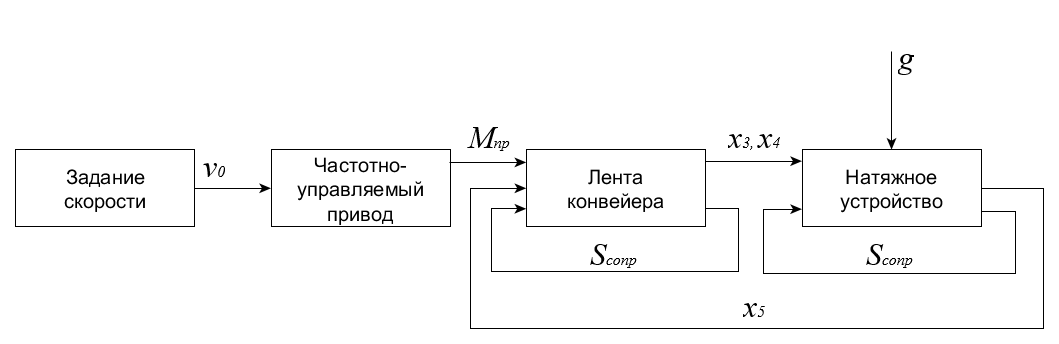
\includegraphics [scale=0.45] {3-6}
  \caption{Структурная схема связи моделей ленты и натяжного устройства, которая обеспечивает возможность управления натяжным устройством} 
  \label{img:3.common_struct}  
\end{figure}

В схеме моделирования, реализованной в Simulink, лента конвейера представлена своей внутренней моделью состояний, параметрами которой являются матрицы $ A $ и $ B $, натяжное устройство представлено своей внешней моделью, реализованной на основе системы уравнений \ref{eq:nu_model}:

\begin{figure} [h!] 
  \center
  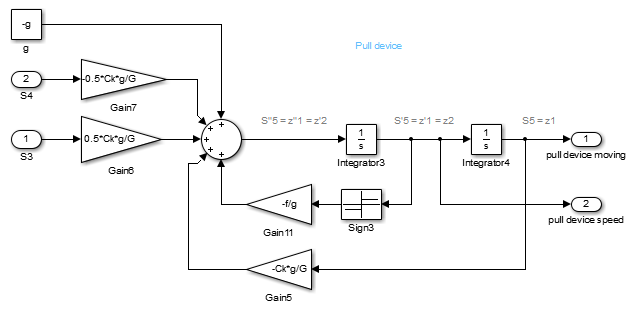
\includegraphics [scale=0.8] {3-7}
  \caption{Структурная схема модели натяжного устройства} 
  \label{img:}  
\end{figure}

\newpage

\if 0
\section{Исследование переходных процессов переключения скорости движения ленты с возникновением проскальзывания} \label{sect3_333}
Проскальзывание ленты конвейера возникает при изменении скорости ее движения. Определить наличие проскальзывания возможно по увеличению разности натяжений в набегающей и сбегающей ветвях конвейера.
Предлагаемая ниже модель конвейера позволяет а измерять возникающие натяжения в любой точке расчетной схемы.

Выполним тяговый расчет конвейера методом обхода по контуру []. Согласно этому методу, натяжения в каждой характерной точке конвейера равно сумме натяжения в предыдущей точке и силы сопротивления движению между этими точками.
На схеме, приведенной на рис.3.4, имеются четыре характерные точки: точки набегания и сбегания ленты на приводной и хвостовой обводной барабаны. 


\fi

\section{Модификация модели конвейера для исследования процессов торможения} \label{sect3_3}

\if 0
Наблюдения за работой ленточных конвейеров показали, что при торможении верхняя ветвь конвейера иногда теряет устойчивость, образуя мешки. При этом наблюдается просыпание груза, а при последующем пуске конвейера лента испытывает повышенные динамические напряжения и груз разбрасывается по сторонам. Поэтому для мощных конвейерных установок, там где это возможно, целесообразно производить остановку за счет свободного выбега, используя тормозные системы только при аварийном торможении

Торможение конвейера представляет собой создание дополнительных тормозных моментов на приводном и хвостовом барабанах, направленных противоположно действующим моментам на барабанах. 
\fi

Останов конвейера может осуществляться как простым отключением привода (свободный выбег), так и с одновременным торможением одного или нескольких барабанов конвейера с помощью тормозных устройств. Второй способ обычно применяется для экстренного торможения конвейера, либо в случае, если свободный выбег занимает значительное время.

При задействовании тормозного устройства на валу барабана, торможение которого производится, возникает дополнительный (тормозной) момент $ M_T $, направленный противоположно направлению движения барабана конвейера. В случае двухбарабанного конвейера имеется возможность прикладывать тормозное усилие как к приводному барабану, так и к хвостовому барабану, поэтому следует рассматривать два тормозных момента $ M_{T \text{пр}} $ и $ M_{T \text{хв}} $ соответственно.

В общей модели конвейера тормозные моменты можно рассматривать как дополнительные управляющие воздействия для модели движения ленты. Для учета этих управляющих воздействий модель, полученную в п.~\ref{sect3_2}, необходимо модифицировать. 

Введем два дополнительных управляющих воздействия. Система дифференциальных уравнений модифицированной модели конвейера с учетом этого записывается следующим образом:

$$ \dot X = \tilde AX + \tilde B_\text{пр}U + \tilde B_\text{ну}U_\text{ну} + \tilde B_s U_s +  \tilde{B_{T \text{пр}}} U_{T \text{пр}} +  \tilde{B_{T \text{хв}}} U_{T \text{хв}}, $$

где $ U_{T \text{пр}} = M_{T \text{пр}}$ -- тормозной момент на приводном барабане,  $ U_{T \text{хв}} = M_{T \text{хв}} $ -- тормозной момент на хвостовом барабане.

Запишем тормозной момент на приводном барабане в матричной форме. Он вычисляется следующим образом $ M_{T \text{пр}} = M^{-1} P_{T \text{пр}} $. Так как этот момент направлен противоположно направлению движения приводного барабана конвейера, то матрица $ P_{T \text{пр}} = -P $.

$$ M_{T \text{пр}} = M^{-1} P_{T \text{пр}} = M^{-1}
	\begin{bmatrix}
	- \frac{1}{R_{\text{б}}} \\
	0                        \\
 	0                        \\
	0                        \\
	0                        \\
	\end{bmatrix}.
 $$
 
Здесь $ R_{\text{б}} $ -- расстояние от оси вала приводного барабана конвейера до точки приложения тормозного усилия (плечо). Примем его равным радиусу приводного барабана для упрощения вычислений. В общем случае оно будет отличаться от радиуса приводного барабана и будет равно радиусу тормозного диска (в случае использования дискового тормозного устройства) или~радиусу тормозного барабана (в случае использования барабанного тормозного устройства).

Аналогично вычисляется второй тормозной момент с учетом его приложения к хвостовому барабану:

$$ M_{T \text{хв}} = M^{-1} P_{T \text{хв}} = M^{-1}
	\begin{bmatrix}
	0                         \\
	0                         \\
	 - \frac{1}{R_{\text{б}}} \\
	0                         \\
	0                         \\
	\end{bmatrix}.
 $$

Рассчитаем матрицу управления модифицированной системы:

$$
\tilde{B_{\text{пр}}}_{[8\times1]} = 
\begin{bmatrix}
 0_{[4\times1]}                      \\
 M^{-1}P_{[4\times1]}                \\
\end{bmatrix},
\tilde{B_{\text{ну}}}_{[8\times8]} = 
\begin{bmatrix}
 0_{[4\times4]} & 0_{[4\times4]}       \\
 0_{[4\times4]} & M^{-1}S_{[4\times4]} \\
\end{bmatrix},
\tilde{B_s}_{[8\times1]} = 
\begin{bmatrix}
 0_{[4\times1]}                      \\
 M^{-1}G_{[4\times1]}                \\
\end{bmatrix}
$$

$$
\tilde{B_{T \text{пр}}}_{[8\times1]} = 
\begin{bmatrix}
 0_{[4\times1]}                      \\
 M^{-1}P_{T1  \quad [4\times1]}      \\
\end{bmatrix},
\tilde{B_{T \text{хв}}}_{[8\times1]} = 
\begin{bmatrix}
 0_{[4\times1]}                      \\
 M^{-1}P_{T2 \quad [4\times1]}       \\
\end{bmatrix}.
$$

Общая матрица управления является конкатенацией описанных выше матриц и имеет размерность $ 8\times12 $:

$$ B_{[8\times12]} = [\tilde{B_{\text{пр}}} \vdots \tilde{B_{\text{ну}}} \vdots \tilde{B_s} \vdots \tilde{B_{T \text{пр}}} \vdots \tilde{B_{T \text{хв}}}]. $$

Размерность вектора управления $ U - 12\times1. $ 

Числовые значения матрицы управления модифицированной системы приведены в приложении \ref{Appendix15}. Программа расчета числовых значений матриц приведена в приложении \ref{Appendix0}.
\\

Так как при исследовании процессов торможения может возникнуть необходимость формировать различные законы изменения тормозных моментов, то целесообразно реализовать модель формирования каждого тормозного момента как отдельную подсистему. Кроме того, необходимо обеспечить правильное направление тормозного момента во всех случаях -- тормозной момент всегда должен быть направлен противоположно направлению движения барабана конвейера. Приведенная на рис.~\ref{img:33.brake} структурная схема удовлетворяет указанным выше требованиям.
\begin{figure} [h!] 
  \center
  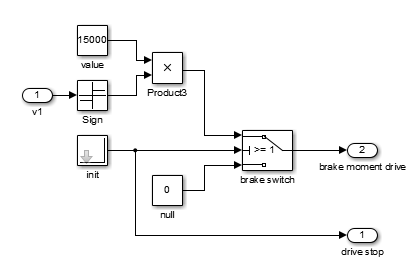
\includegraphics [scale=0.8] {33-1.png}
  \caption{Структурная схема модели формирования тормозного момента.} 
  \label{img:33.brake}  
\end{figure}

На этой схеме блок \textit{init} определяет моменты времени для включения и отключения тормозного устройства, блок \textit{brake swith} обеспечивает изменение значения соответствующего управляющего воздействия для модели движения ленты (выход \textit{brake moment drive}) с нулевого на значение, меняющееся по предварительно заданному закону. В данном случае это скачкообразное изменение значения тормозного момента до $ 15000 H $. На вход \textit{v1} подается текущее значение скорости барабана конвейера, а блок \textit{sign} на выходе формирует значение $1$, если скорость положительна, и значение $-1$, если скорость отрицательна. Блок \textit{drive stop} служит для~формирования управляющего воздействия для отключения привода конвейера.
\\

Таким образом уточненная модель конвейера отличается наличием двух дополнительных управляющих воздействий -- тормозных моментов, наличием подсистем формирования тормозных моментов и возможностью отключения привода конвейера. В дальнейшем будем моделировать процессы торможения конвейера посредством задания законов изменения значений тормозных моментов в функции времени.

\section{Вычисление натяжений ленты конвейера и тягового фактора} \label{sect3_4}
Одним из требуемых условий нормальной работы конвейерной установки является условие отсутствия проскальзывания ленты на барабанах во всех режимах работы. Это условие определяется уравнением Эйлера, которое записывается в следующем виде.

Для случаев пуска конвейера и переключения с меньшей скорости на большую:
$$ \frac{S_{\text{наб}}}{S_{\text{сб}}} \leqslant E^{\mu \alpha}, $$

Для случаев торможения конвейера и переключения с большей скорости на меньшую:

$$ \frac{S_{\text{сб}}}{S_{\text{наб}}} \leqslant \frac{1}{E^{\mu \alpha}}, $$

где $ e^{\mu \alpha} $ -- тяговый фактор ленточного конвейера, $ S_{\text{наб}} $ -- натяжение в точке набегания ленты на~барабан, \textit{Н}, $ S_{\text{сб}} $ -- натяжение в точке сбегания ленты с барабана, \textit{Н}.

Здесь $ e $ -- основание натурального логарифма;
      $ \mu $  -- коэффициент трения скольжения между лентой и барабаном;
      $ \alpha $ -- угол обхвата барабана лентой, рад.
      
Коэффициент трения скольжения между лентой и барабаном определяется по технологическим таблицам \cite{lshakhmeyster} и зависит от поверхности приводного барабана, состояния соприкасающихся поверхностей, атмосферных условий. Для конвейера с одним приводом, с футеровкой барабана резиной, при влажной погоде и загрязнении поверхностей ленты и барабана углем, песком и~глиной коэффициент сцепления $ \mu = 0,25 $. Для конвейера с одним приводом угол охвата барабана лентой примем $ \alpha = \pi $. При этих условиях величина тягового фактора при пуске конвейера и при переключении с меньшей скорости на большую не должна превышать $ e_0^{\mu \alpha} = 2,5 $, при~торможении конвейера величина тягового фактора не должна превышать $ \frac{1}{e_0^{\mu \alpha}} = 0,4 $

Ниже описано измерение возникающих натяжений в любой точке расчетной схемы, показанной на рис.~\ref{img:3.sheme}. На основе данных измерений можно вычислять текущее значение тягового фактора для определения наличия проскальзывания ленты конвейера.

Натяжения в характерных точках расчетной схемы будем определять на основании измерения деформаций различных участков конвейерной ленты, которые вызваны усилиями в ленте. Сначала составим структурную схему вычисления натяжений в точке набегания ленты на приводной барабан и в точке сбегания ленты с приводного барабана. Для этого необходимо определить связь между деформацией и натяжением в характерных точках 1 и 4 посредством "тарирования" ленты конвейера. Рассчитаем натяжения $ S_1, S_2, S_3, S_4 $ (рис.~\ref{img:3.schema_forces}) при весе груза натяжного устройства (или натяжении в канате натяжной каретки автоматического натяжного устройства), равного $ G_{\text{ну}} $.

В модели конвейера меняем вес груза и, фиксируя возникающие деформации, ставим им в~соответствие рассчитанные натяжения $ S_1 $ и $ S_4 $.

В работе \cite{vdmitrieva} отмечено, что груз натяжного устройства своим весом $ G_{\text{ну}} $ создает в точках 2~и~3 натяжения $ S_2 $ и $ S_3 $, приблизительно равные $ 0,5 G_{\text{ну}} $.

Тогда натяжения $ S_1 $ и $ S_4 $ соответственно равны:

$$ S_1 = 0,5 G_{\text{ну}} + W_{\text{гр}}, $$
$$ S_4 = 0,5 G_{\text{ну}} - W_{\text{п}}, $$

где $ W_\text{гр} $ и $ W_\text{п} $ сопротивления движению грузовой и порожней ветвей соответственно, которые равны:

\begin{equation}
\label{eq:wgr}
 W_{\text{гр}} = q_{\text{гр} \Sigma} l w,
\end{equation}

\begin{equation}
\label{eq:wp}
W_{\text{п}} = q_{\text{п} \Sigma} l w.
\end{equation}

\begin{figure} [h!] 
  \center
  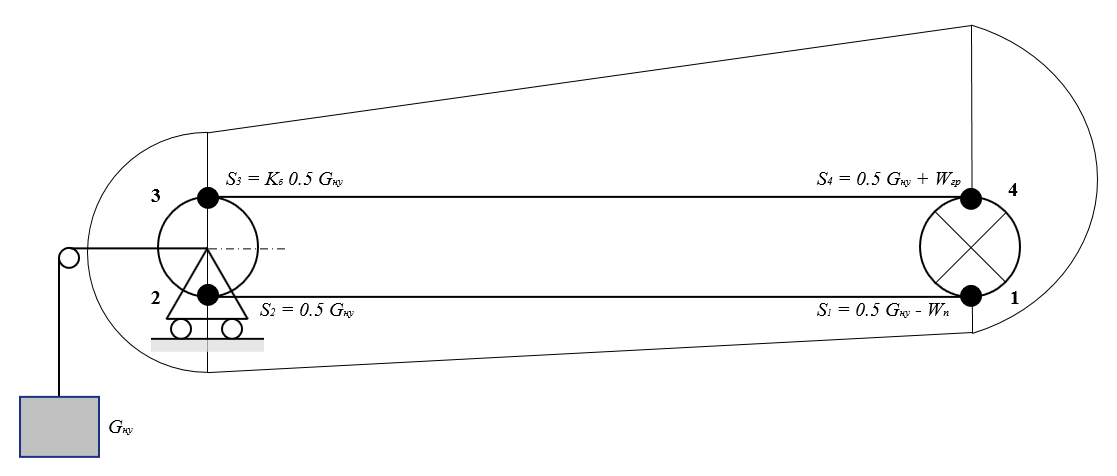
\includegraphics [scale=0.4] {3-4.png}
  \caption{Определение натяжений в конвейерной ленте.} 
  \label{img:3.schema_forces}  
\end{figure}

Здесь $ l $ -- длина конвейера, $ q_{\text{гр} \Sigma} = q_{\text{л}} + q_{\text{р}} + q_{\text{гр}} = 1040 \text{Н/м} $ -- суммарный погонный вес грузовой ветви, равный сумме веса отрезка ленты грузовой ветви, веса роликоопор грузовой ветви и веса груза на ленте, $ q_{\text{п} \Sigma} = q_{\text{л}} + q\prime_{\text{р}} = 250 \text{Н/м} $ -- суммарный погонный вес порожней ветви, равный сумме веса отрезка ленты порожней ветви и веса роликоопор порожней ветви, $ w $ -- коэффициент сопротивления движению ленты, который определяется по технологическим таблицам \cite{izapenin2,vdmitriev2}. Для хорошего состояния конвейера, для стационарных или полустационарных установок, при~небольшом загрязнении ленты $ w = 0.03 $. Тогда сопротивление движению грузовой ветви равно

$$ W_{\text{гр}} = 1040 \cdot 1000 \cdot 0,03 = 31215 H. $$

Сопротивление движению порожней ветви равно

$$ W_{\text{п}} = 250 \cdot 1000 \cdot 0,03 = 7500 H. $$

Рассчитаем натяжения $ S_1 $ и $ S_4 $, возникающие в точках набегания и сбегания ленты конвейера на приводной барабан, при различном весе груза натяжного устройства $ G_{\text{ну}} $. Этим натяжениям соответствуют деформации $ x_1 - x_2 $ и $ x_4 - x_1 $, которые измеряются в модели.

Результаты вычисления величин натяжений, а также результаты измерения натяжений представлены в табл.~\ref{tabl:resultS}.

\begin{table}[h!]
\caption{Результаты расчета натяжений ленты при различных значениях веса натяжного устройства и соответствующие им деформации.}
\label{tabl:resultS}

\begin{center}
\begin{tabular}{|p{0.2\linewidth}|l|l|l|l|l|l|p{0.1\linewidth}|p{0.1\linewidth}|}
\hline
Вес груза натяжного устройства $ G_{\text{ну}}, H $ & $ x_1 - x_2 $ & $ x_2 - x_3 $ & $ x_3 - x_4 $ & $ x_4 - x_1 $ & $ S_4, H $ & $ S_1, H $ & Тяговый фактор $S_1 / S_4 $ \\
\hline
20000 & 4,25  & 2,69  & -8,28  & 1,34 & 2500  & 41200 & 16,48 \\
\hline
30000 & 5,50  & 3,94  & -12,03 & 2,59 & 7500  & 46200 & 6,16  \\
\hline
40000 & 6,76  & 5,19  & -15,80 & 3,85 & 12500 & 51200 & 4,10  \\
\hline
50000 & 8,01  & 6,44  & -19,55 & 5,10 & 17500 & 56200 & 3,21  \\
\hline
55000 & 8,64  & 7,07  & -21,43 & 5,72 & 20000 & 58700 & 2,94  \\
\hline
60000 & 9,26  & 7,69  & -23,30 & 6,35 & 22500 & 61200 & 2,72  \\
\hline
65000 & 9,88  & 8,31  & -25,16 & 6,99 & 25000 & 63700 & 2,55  \\
\hline
70000 & 10,50 & 8,94  & -27,03 & 7,59 & 27500 & 66200 & 2,41  \\
\hline
75000 & 11,12 & 9,56  & -28,89 & 8,21 & 30000 & 68700 & 2,29  \\
\hline
80000 & 11,74 & 10,18 & -30,75 & 8,83 & 32500 & 71200 & 2,19  \\
\hline
85000 & 12,36 & 10,80 & -32,61 & 9,45 & 35000 & 73700 & 2,11  \\
\hline
\end{tabular}
\end{center}
\end{table}


На основе данных табл.~\ref{tabl:resultS} определим зависимость между деформацией $ \delta_1 $ участка $ x_1 - x_2 $ и~натяжением $ S_1 $, возникающем в точке набегания ленты на приводной барабан:
\begin{equation}
\label{eq:s1}
S_1 = f(\delta_1) = 4006,9 \delta_1 + 24130,5.
\end{equation}

Зависимость между деформацией $ \delta_4 $ участка $ x_4 - x_1 $ и натяжением $ S_4 $, возникающем в точке сбегания ленты с приводного барабана:

\begin{equation}
\label{eq:s4}
S_4 = g(\delta_4) = 4005,6 \delta_4 - 2904,7.
\end{equation}

Графики зависимостей представлены на рис.~\ref{img:3.s1s4} (а, б). Определение зависимостей производилось в программном комплексе Matlab с использованием метода наименьших квадратов. Исходный код расчета представлен в приложении \ref{AppendixLSM}.

\begin{figure}[h]
  \begin{minipage}[h]{0.49\linewidth}
    \center{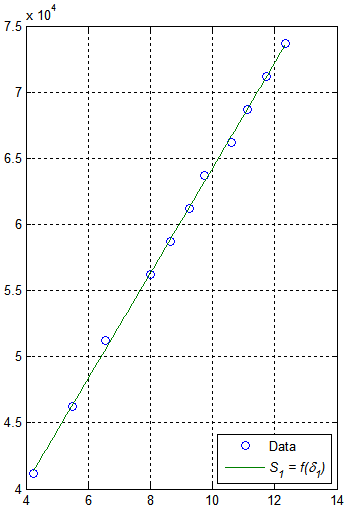
\includegraphics[width=1\linewidth]{3-13.png} \\ а)}
  \end{minipage}
  \hfill
  \begin{minipage}[h]{0.49\linewidth}
    \center{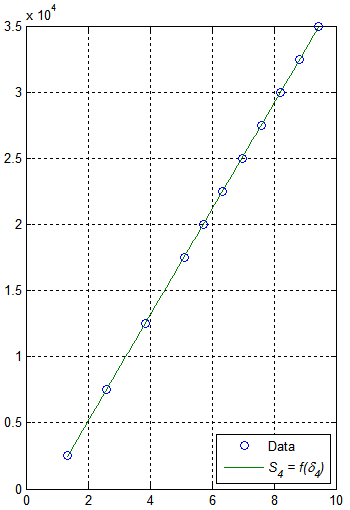
\includegraphics[width=1\linewidth]{3-14.png} \\ б)}
  \end{minipage}
  \caption{Графики зависимости натяжений в ветвях конвейера от деформации участков}
  \label{img:3.s1s4}  
\end{figure}

Располагая зависимостями $ f(\delta_1) $ и $ g(\delta_4) $, становится возможным при изменяющихся деформациях $ \delta_1 $ и $ \delta_4 $ непрерывно вычислять натяжения $ S_1 $ и $ S_4 $ и значения тягового фактора.\\

Величина тягового фактора при разгоне конвейера и при переключении с меньшей скорости на большую:

$$ E^{\mu \alpha}(t) = \frac{S_1(t)}{S_4(t)} $$

Величина тягового фактора при торможении конвейера и при переключении с большей скорости на меньшую:

$$ \frac{1}{E^{\mu \alpha}(t)} = \frac{S_4(t)}{S_1(t)} $$

Структурная схема определения деформаций ленты, вычисления величин натяжений и тягового фактора представлена на рис.~\ref{img:3.ema}.

\begin{figure} [h!] 
  \center
  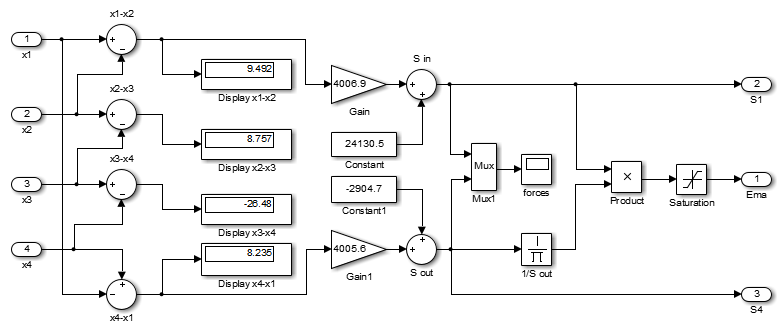
\includegraphics [scale=0.8] {3-15.png}
  \caption{Структурная схема определения деформаций ленты, вычисления величин натяжений и тягового фактора} 
  \label{img:3.ema1}  
\end{figure}

\clearpage

\section{Моделирование различных режимов работы ленточного конвейера с натяжным устройством, расположенным в хвостовой части} \label{sect3_5}
Компьютерное моделирование производилось в системе SIMULINK, входящей в пакет прикладных программ MATLAB. Этот программный продукт позволяет выполнять моделирование динамических систем, описываемых обыкновенными нелинейными дифференциальными уравнениями. Структурная схема системы, включающей в себя контур ленты конвейера и натяжное устройство, была реализована с использованием типовых блоков SIMULINK.

Математической моделью ленточного конвейера как технологического объекта является объединение модели ленты с восемью координатами состояния, характеризующими кинематику перемещения четырех сосредоточенных масс, модели натяжного устройства и модели управляемого асинхронного электропривода. 

Схема общей модели конвейера представлена на рис.~\ref{img:3.common}. Модель системы разбита на подсистемы, каждая из которых представляет собой определенный узел конвейерной установки: модель ленты конвейера, модель натяжного устройства, модель асинхронного короткозамкнутого привода, модель задатчика скорости, модели задатчиков тормозных моментов. На данном этапе моделирование производится без каких-либо регулирующих воздействий. Целью моделирования является получение переходных процессов сосредоточенных масс ленты конвейера при пуске, переключении скоростей, свободном выбеге и торможении.

\begin{figure} [h] 
  \center
  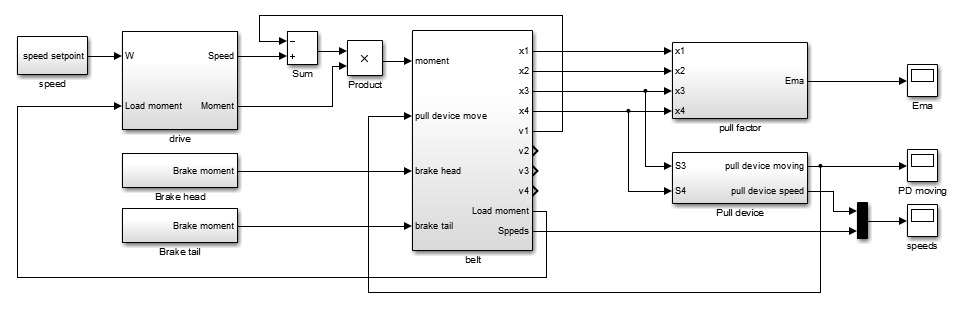
\includegraphics [scale=0.7] {3-8.png}
  \caption{Общая схема моделирования конвейерной установки.} 
  \label{img:3.common}  
\end{figure}

Здесь блок \textit{Drive} -- асинхронный короткозамкнутый привод, Блок \textit{Speed} -- задатчик скорости привода, блоки \textit{Brake head} и \textit{Brake tail} -- формирователи тормозных моментов для головного и~хвостового барабанов соответственно, блок \textit{Pull factor} -- вычисление величины тягового фактора, блок \textit{Pull device} -- модель натяжного устройства, структурная схема которой представлена на рис. 3.6, блок \textit{Belt} -- модель ленты конвейера, которая  представлена своей внутренней моделью:

$$ \dot x = Ax + Bu, $$
$$ y = Cx + Du. $$ 

Структурная схема модели ленты представлена на рис.~\ref{img:3.belt}.

\begin{figure} [h] 
  \center
  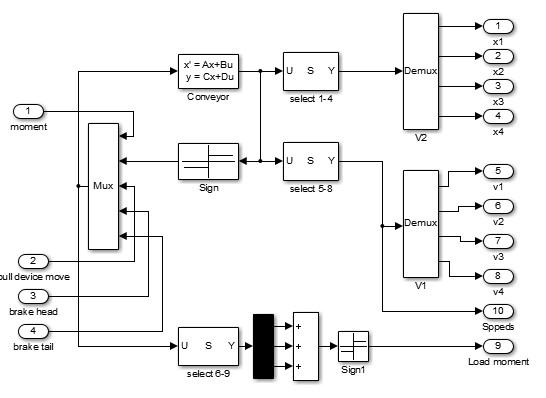
\includegraphics [scale=0.8] {3-9.png}
  \caption{Структурная схема модели ленты конвейера.} 
  \label{img:3.belt}  
\end{figure}

Для реализации управления пять внешних воздействий -- момент, создаваемый приводом, силы сопротивления движению сосредоточенных масс ленты, усилие, создаваемое весом натяжного устройства и два тормозных момента объединены в один вектор $ U $, размерность которого $ 14 \times 1 $. Матрица $ B = [B_1 \vdots B_2 \vdots B_3] $, размерность матрицы $ B - 10 \times 14$. Матрица $ D $ -- нулевая. В качестве выходных сигналов рассматриваются скорости движения сосредоточенных масс, поэтому матрица $ C = [0 \quad 0 \quad 0 \quad 0 \quad 0 \quad 1 \quad 1 \quad 1 \quad 1 \quad 1] $. 

Модель привода представляет собой модель электрической асинхронной машины со своей собственной системой управления, описанной в \cite{vdmitrieva}.\\

Для связи моделей ленты и привода необходимо:
\begin{itemize}
\item вычислить момент нагрузки $ M_H $, приведенный к валу двигателя, который определяется силами сопротивления движению конвейерной ленты. Для технологической схемы с натяжным устройством, расположенным в хвосте конвейера, расчет производится следующим образом:
$$ F_{\text{сопр}} = 0,5 (G_{\text{г}} + G_{\text{п}}) l w \text{sgn} \dot x_1 + G_{\text{г}} l w \text{sgn} \dot x_2 + 0,5 (G_{\text{г}} + G_{\text{п}}) l w \text{sgn} \dot x_3 + G_{\text{п}} l w \text{sgn} \dot x_4; $$
\item в модели привода выполнить переход от моделирования в условном времени к моделированию в реальном времени для согласования параметров моделирования двух подсистем;
\item в качестве управляющего сигнала в модель ленты подается движущий момент привода $ M, $ а в качестве задающего сигнала - скорость вращения ротора $ \omega $;
\item так как моделирование привода проводится в нормированных единицах, необходимо умножить сигнал момента на коэффициент, равный номинальному моменту выбранного привода $ M_{\text{ном}} $.
\end{itemize}

Будем моделировать прямой пуск конвейера, последующее его движение с постоянной скоростью $ v_1 = 1 \text{ м/с} $, переключение на скорость $ v_2 = 2 \text{ м/с} $, последующее переключение на скорость $ v_1 $ и останов со свободным выбегом.

Результатами моделирования являются:
\begin{itemize}
\item переходные процессы по моменту привода и частоте его вращения, приведенные на~рис.~\ref{img:3.mv};
\item переходные процессы по скоростям обобщенных координат ленты, представленные на~рис.~\ref{img:3.pp};
\item переходные процессы по скорости натяжного устройства, представленные на рис.~\ref{img:3.nu};
\item переходные процессы по перемещению каретки натяжного устройства, представленные на~рис.~\ref{img:3.pdx};
\item переходные процессы по изменению величины тягового фактора, представленные на~рис.~\ref{img:3.ema}.
\end{itemize}

\begin{figure} [h!] 
  \center
  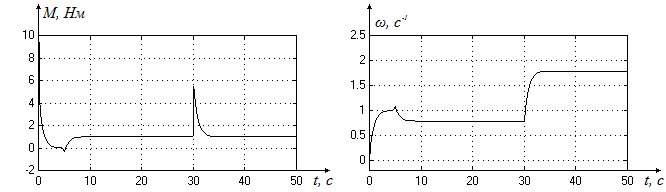
\includegraphics [scale=1] {3-2.png}
  \caption{Изменение момента, развиваемого двигателем и частоты вращения ротора.} 
  \label{img:3.mv}
\end{figure}

\begin{figure} [h!] 
  \center
  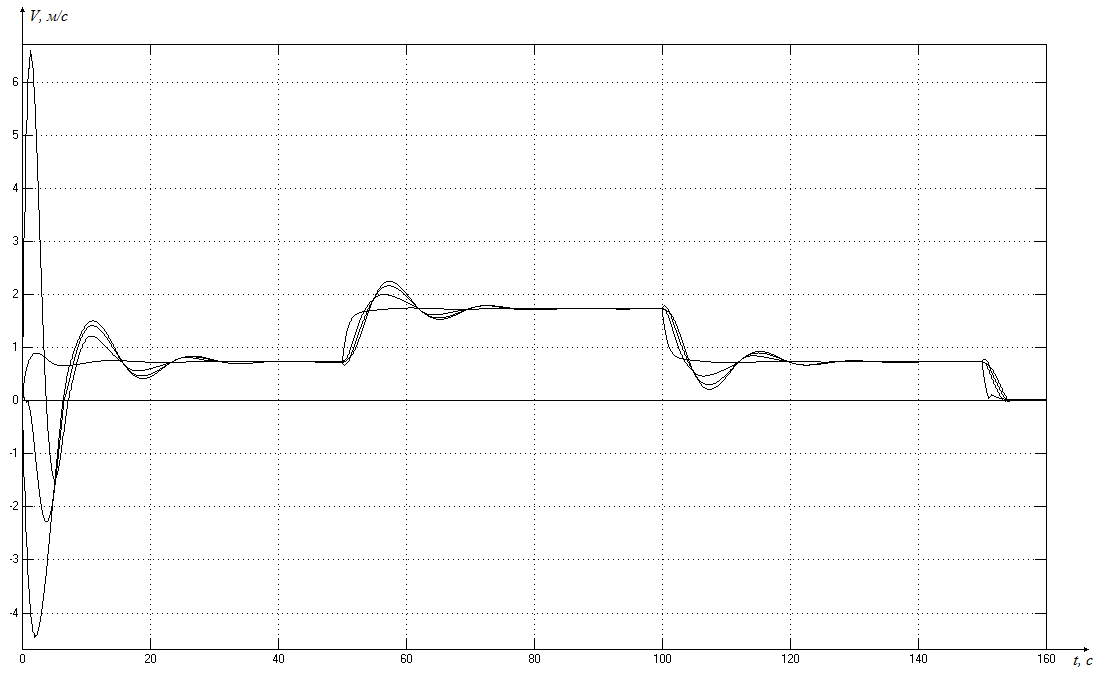
\includegraphics [scale=0.6] {3-3.png}
  \caption{Переходные процессы по скоростям обобщенных координат ленты конвейера.} 
  \label{img:3.pp}  
\end{figure}

\begin{figure} [h!] 
  \center
  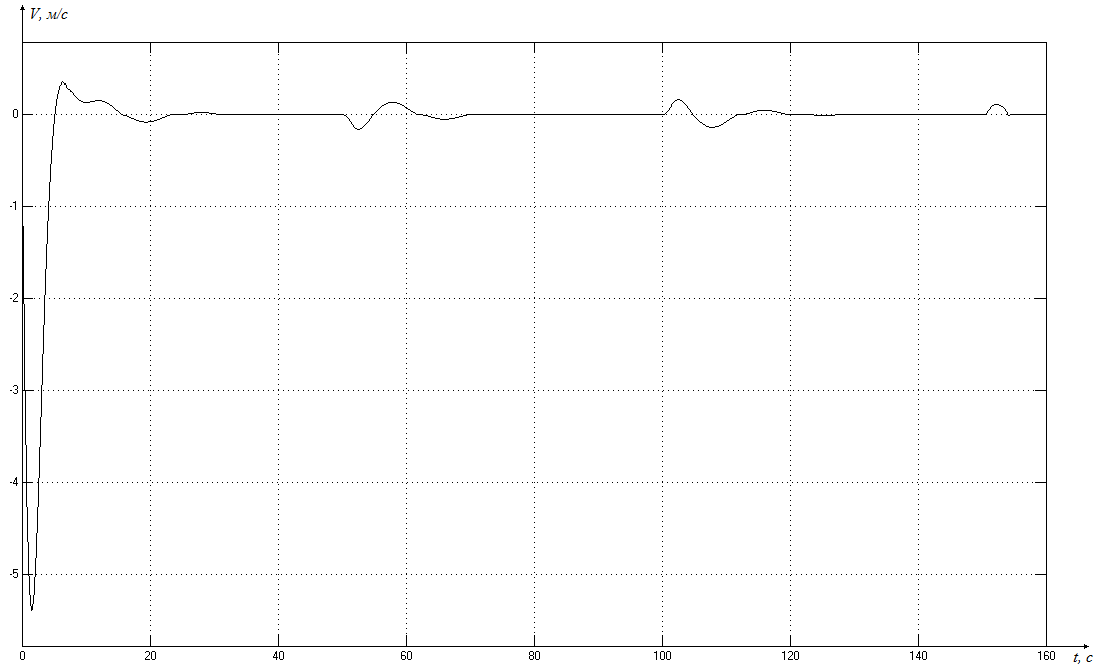
\includegraphics [scale=0.6] {3-10.png}
  \caption{Переходной процесс по скорости перемещения каретки натяжного устройства конвейера.} 
  \label{img:3.pd}  
\end{figure}

\begin{figure} [h!] 
  \center
  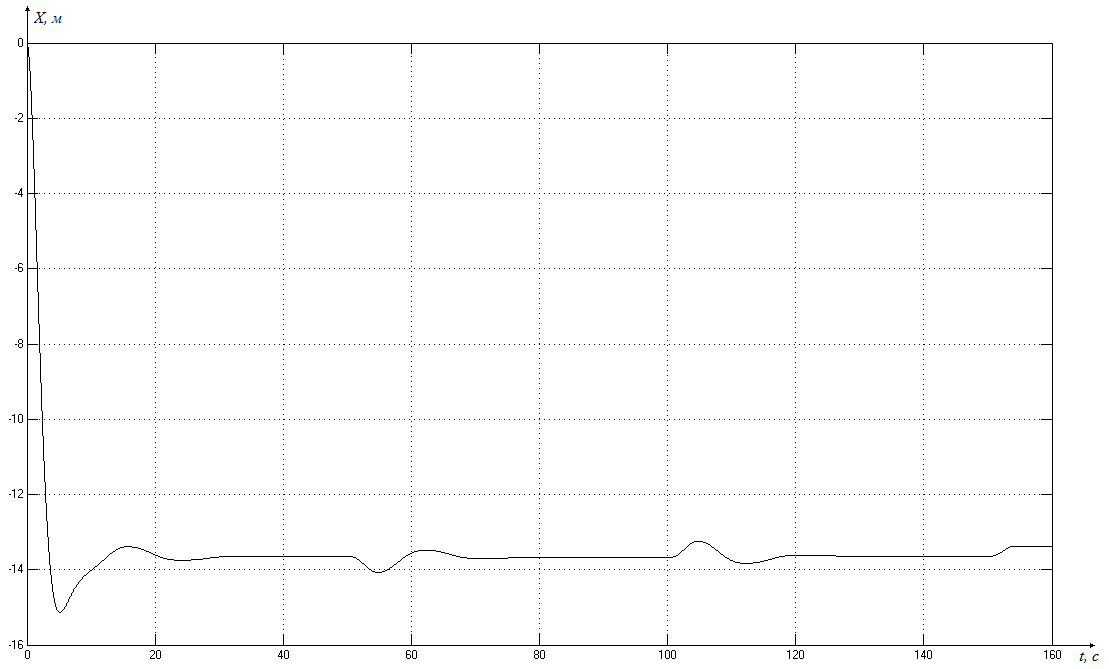
\includegraphics [scale=0.6] {3-11.png}
  \caption{Переходной процесс по перемещению каретки натяжного устройства конвейера.} 
  \label{img:3.pdx}  
\end{figure}
\clearpage

\begin{figure} [h!] 
  \center
  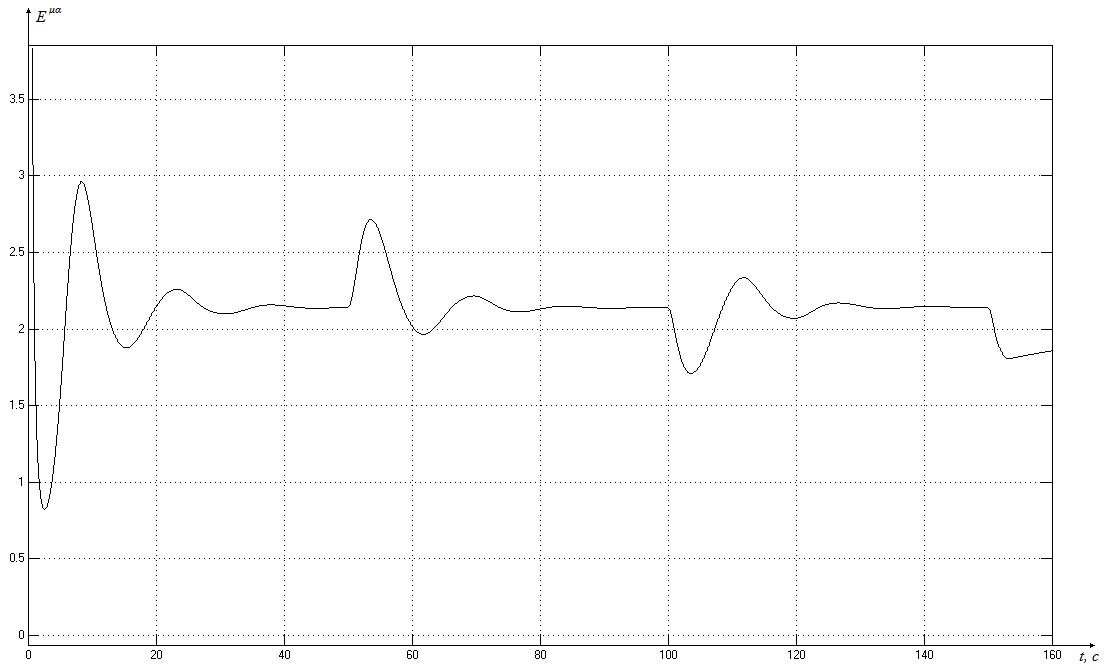
\includegraphics [scale=0.6] {3-12.png}
  \caption{Изменение величины тягового фактора.} 
  \label{img:3.ema}  
\end{figure}

Ниже представлен более подробный анализ следующих переходных процессов и описаны особенности каждого из них:
\begin{itemize}
\item пуск конвейера;
\item переключение на большую скорость движения ленты;
\item переключение на меньшую скорость движения ленты;
\item останов конвейера без торможения (свободный выбег);
\item останов конвейера с торможением приводного барабана;
\item торможение приводного и натяжного барабанов в произвольные моменты времени.
\end{itemize}

\subsection{Пуск конвейера и переключение с меньшей скорости на большую} \label{subsect3_5_1}
Пуск конвейера характеризуется появлением динамических натяжений в ленте, которые, алгебраически суммируясь со статическими натяжениями, изменяют результирующие натяжения ленты и усилия в элементах конвейера. Эти изменения могут привести к неустойчивой работе приводного барабана -- к частичному или полному проскальзыванию. Проскальзывание недопустимо по нескольким причинам -- изнашивание футеровки барабана становится более интенсивным, происходит нагрев барабана, снижение коэффициента сцепления. Анализ процесса пуска конвейера позволяет оценить параметры переходных процессов, определить экстремальные значения натяжений, оценить влияние на них параметров конвейера, а также определить алгоритмы управления и методы, необходимые для оптимизации переходных процессов.

Пуск конвейера обычно осуществляется в три этапа. Первый этап -- вывод на ползучую скорость ($0,2$ м/с); второй этап -- движение ленты на ползучей скорости и ожидание завершения переходных процессов, являющихся следствием упругих деформаций в ленте; третий этап -- вывод на рабочую скорость.

Ниже представлены графики переходных процессов по скоростям сосредоточенных масс ленты и натяжного устройства (рис.~\ref{img:3.speeds}), изменение натяжений в точках набегания ленты на~приводной барабан и сбегания ленты с приводного барабана (рис.~\ref{img:3.forces}), а также изменение величины тягового фактора рис.~\ref{img:3.ema} и перемещение натяжного устройства (рис.~\ref{img:3.pd}) при пуске конвейера с выводом на ползучую скорость $0,2$ м/с и переключением на рабочую скорость $1,2$ м/с через $40$ секунд.

Переходные процессы по скоростям сосредоточенных масс конвейера отличаются довольно высокой колебательностью и длительным временем регулирования порядка $30$ сек при выводе на ползучую скорость и порядка $20$ сек при выводе на номинальную скорость. В движении массы $ m_2 $, расположенной в центре грузовой ветви, и массы $ m_3 $, расположенной на хвостовом барабане, в момент пуска конвейера и в момент переключения скорости наблюдается перемещение в~сторону, противоположную основному движению конвейера, что связано с перемещением натяжного устройства под действием силы тяжести, отводящего хвостовой барабан назад вследствие уменьшения натяжения ленты на порожней ветви.

Колебательные переходные процессы негативно влияют на срок службы ленты, увеличивают ее износ. По этой причине при расчете и проектировании конвейера приходится выбирать более дорогие ленты с увеличенным запасом прочности, что экономически невыгодно.


Изменение натяжений также носит колебательный характер, а величина тягового фактора в~определенные моменты времени превышает значение $2,5$. Это означает, что при пуске конвейера и при переключении скорости условие Эйлера не выполняется и возникает проскальзывание ленты на приводном барабане. На основании рис.~\ref{img:3.ema} можно видеть, что проскальзывание возникает в следующие моменты времени:
\begin{itemize}
\item через $6,6$ сек после пуска конвейера продолжительностью $4$ сек;
\item через $1,5$ сек после переключения на повышенную скорость продолжительностью $4,4$ сек.
\end{itemize}

Задача стабилизации тягового фактора при пуске конвейера и при переключении скорости движения ленты с меньшей на большую успешно решена в работах \cite{vdmitrieva} и \cite{sgershun}. В работе \cite{sgershun} была получена модель автоматической стабилизации величины тягового фактора магистрального конвейера с двухдвигательным приводом. Автоматическая стабилизация осуществляется регулированием положения каретки натяжного устройства. В работе \cite{vdmitrieva} получена аналогичная модель автоматической системы стабилизации тягового фактора для двух типов однодвигательных конвейеров~--- с натяжным устройством, расположенным в головной части и с натяжным устройством, расположенном в хвостовой части. В обеих работах рассматривались только случаи переключения скорости движения ленты с меньшей на большую и не рассматривались процессы останова и торможения конвейера.

Полученные в работах \cite{vdmitrieva} и \cite{sgershun} модели автоматических систем используются в технической реализации комплексной системы автоматического управления, описываемой в настоящей работе.

\begin{figure} [h] 
  \center
  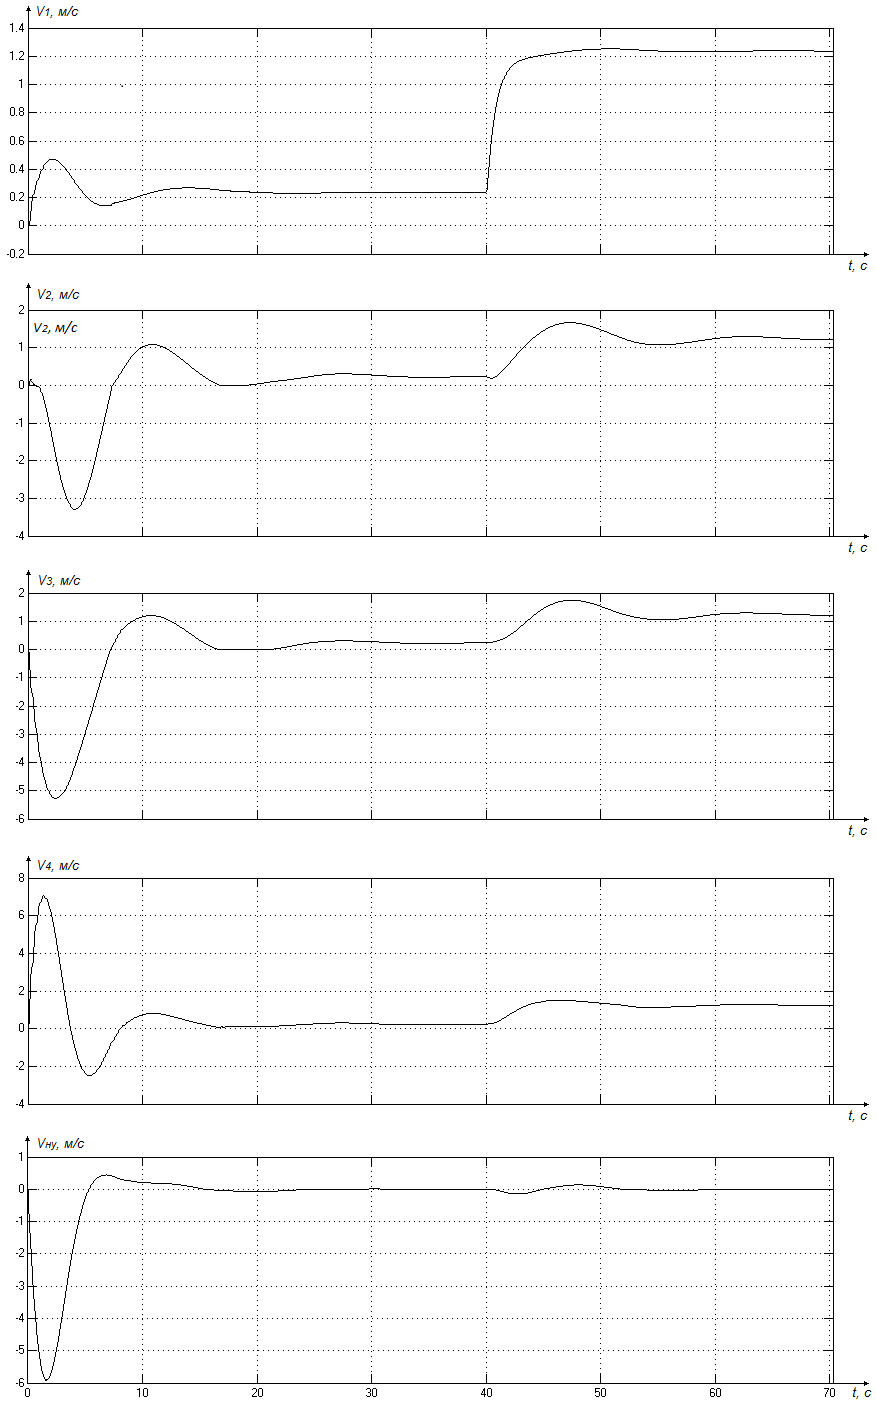
\includegraphics [scale=0.7] {351-1.png}
  \caption{Переходные процессы по скоростям сосредоточенных масс ленты и натяжного устройства при пуске конвейера} 
  \label{img:3.speeds}  
\end{figure}

\begin{figure} [h] 
  \center
  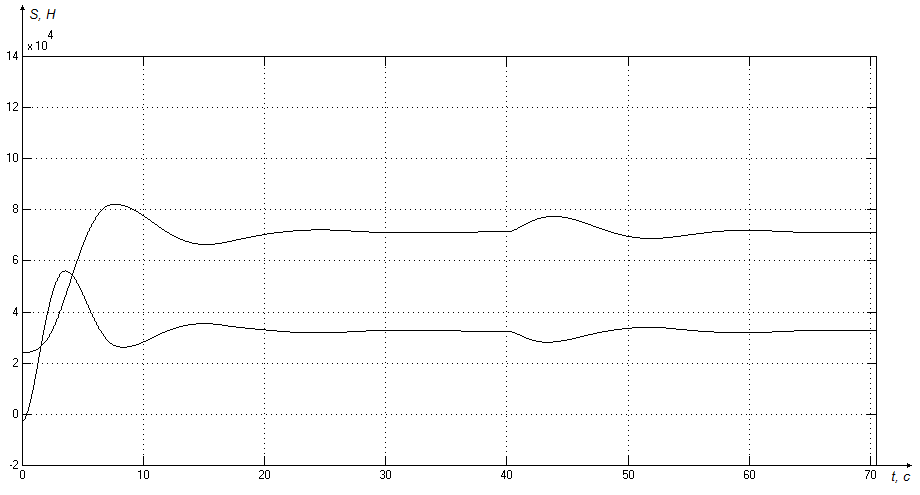
\includegraphics [scale=0.65] {351-2.png}
  \caption{Изменение натяжений в точках набегания ленты на приводной барабан и сбегания ленты с приводного барабана} 
  \label{img:3.forces}  
\end{figure}

\begin{figure} [h] 
  \center
  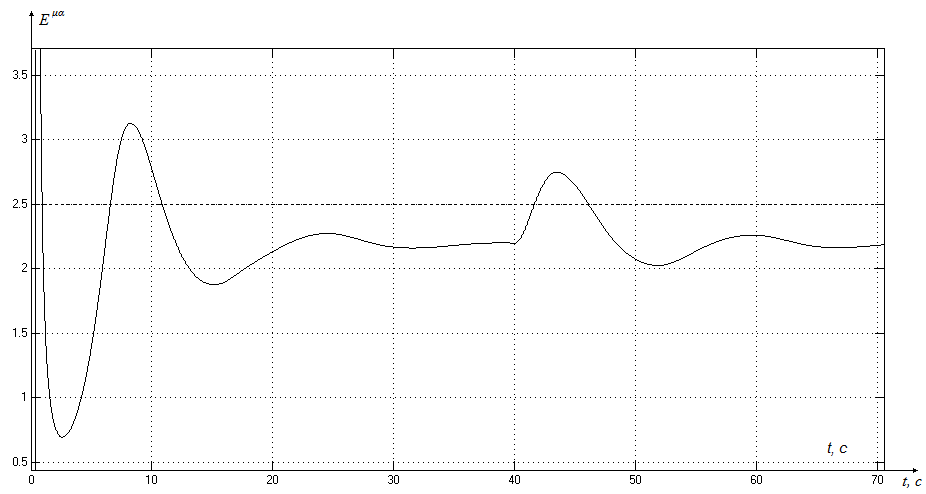
\includegraphics [scale=0.65] {351-3.png}
  \caption{Изменение величины тягового фактора} 
  \label{img:3.ema11}  
\end{figure}

\clearpage

\begin{figure} [h] 
  \center
  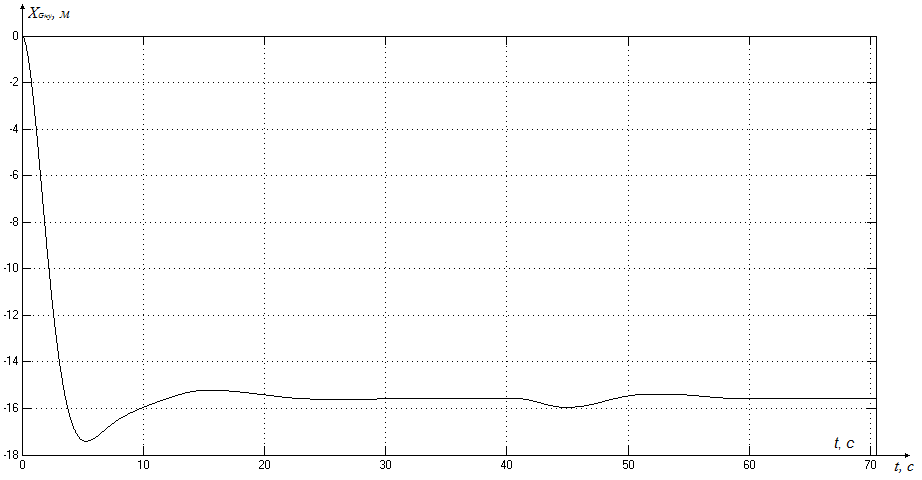
\includegraphics [scale=0.65] {351-4.png}
  \caption{Перемещение натяжного устройства} 
  \label{img:3.nu}  
\end{figure}


\subsection{Останов конвейера без использования торможения (свободный выбег)} \label{subsect3_5_2}
При останове и торможении конвейера также возникают дополнительные динамические натяжения, которые приводят к неустойчивой работе установки во время торможения. При отключении привода также может возникать проскальзывание ленты конвейера. Анализ процесса останова конвейера позволяет оценить параметры переходных процессов, определить максимально допустимые усилия тормозных устройств, обеспечивающих экстренное торможение, определить натяжение грузовой ветви, при котором не происходит потеря ее поперечной устойчивости, определить требования к алгоритмам и методам управления, необходимым для оптимизации переходных процессов останова и торможения.

Рассмотрим останов конвейера без применения торможения (свободный выбег). Технологически эта операция осуществляется отключением привода. После отключения лента некоторое продолжает движение под действием сил инерции, скорость движения постепенно уменьшается. Проведем моделирование останова конвейера при скорости движения ленты, равной $1,2$ м/с. На рис.~\ref{img.3.brake1} представлены графики переходных процессов по скоростям сосредоточенных масс ленты и натяжного устройства в этом случае.

Из рис.~\ref{img.3.brake1} видно, что что скорость первой сосредоточенной массы, находящейся в точке набегания ленты на приводной барабан, падает по экспоненциальному закону. Падение скоростей остальных сосредоточенных масс происходит медленнее за счет наличия упругих деформаций в~ленте конвейера. Все переходные процессы завершаются на $5$ секунд.

Натяжное устройство в момент отключения привода начинает движение и перемещается примерно на $0,5$ м, что объясняется падением натяжений в ленте конвейера.

На рис.~\ref{img.3.brake2} представлено изменение натяжений в точках набегания ленты на приводной барабан и сбегания ленты с приводного барабана, на рис.~\ref{img.3.brake3} представлено изменение величины тягового фактора, вычисленное по формуле () на основе измеренных значений натяжений.

При останове конвейера без применения тормозных устройств в момент отключения привода натяжение в точке набегания ленты на приводной барабан $ S_\text{наб} $ уменьшается на величину $ 7060H, $ натяжение в точке сбегания ленты с приводного барабана $ S_\text{сб} $ увеличивается на величину $ 4540H $. Результирующее значение тягового фактора для режима торможения, равное $ \frac{S_\text{сб}}{S_\text{наб}} $, увеличивается и превышает значение $0,4$, что говорит о наличии проскальзывания ленты конвейера на протяжении всего времени останова. 

\begin{figure} [h] 
  \center
  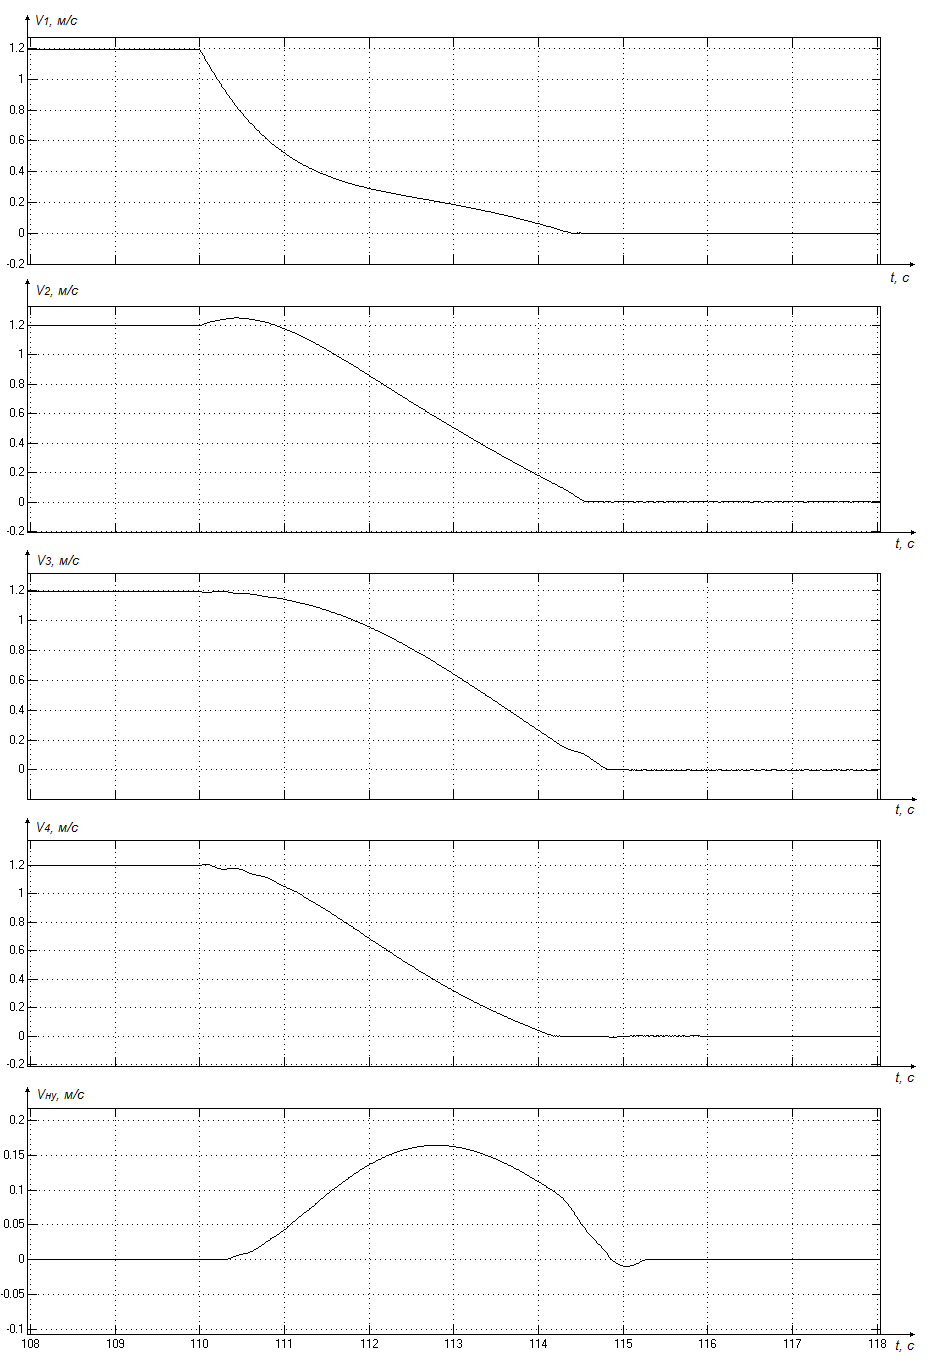
\includegraphics [scale=0.51] {352-1.png}
  \caption{Переходные процессы по скоростям сосредоточенных масс ленты и натяжного устройства при останове конвейера без применения торможения} 
  \label{img.3.brake1}  
\end{figure}

\begin{figure} [h] 
  \center
  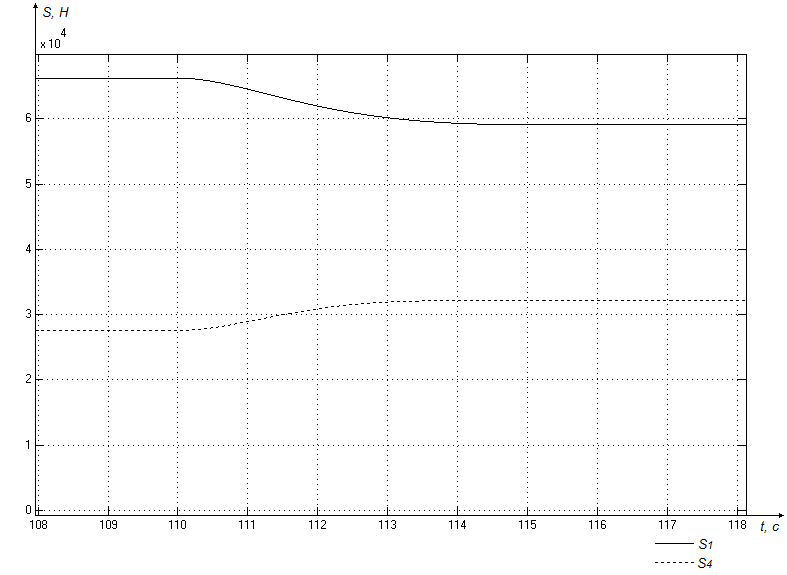
\includegraphics [scale=0.75] {352-2.png}
  \caption{Изменение натяжений в точках набегания ленты на приводной барабан и сбегания ленты с приводного барабана при останове конвейера без применения торможения} 
  \label{img.3.brake2}  
\end{figure}

\begin{figure} [h] 
  \center
  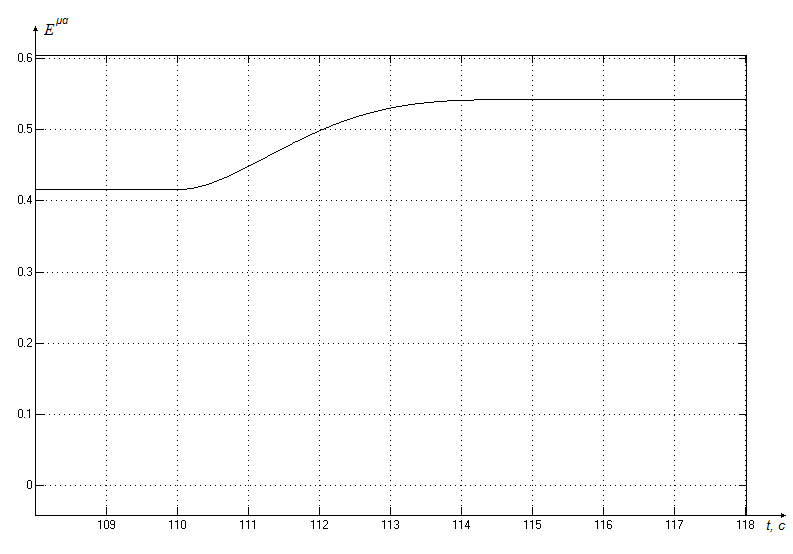
\includegraphics [scale=0.75] {352-3.png}
  \caption{Изменение величины тягового фактора при останове конвейера без применения торможения} 
  \label{img.3.brake3}  
\end{figure}
\clearpage

Следует обратить особое внимание на то, что значение тягового фактора для режима торможения превышает значение $0,4$ на протяжении всего времени работы конвейера. Это показывает, что останов конвейера в любой момент времени будет сопровождаться проскальзыванием ленты. Одним из вариантов решения проблемы проскальзывания ленты при останове могло бы быть уменьшение значения тягового фактора для режима торможения во время работы конвейера, что может быть достигнуто, например, уменьшением веса натяжного устройства. Однако, связь тягового фактора для режима торможения и тягового фактора для режима пуска и разгона не~позволяет уменьшить значение первого параметра без увеличения второго. Это подтверждается экспериментальными данными.

Экспериментально было установлено, что для конвейера с выбранными параметрами вес натяжного устройства, равный $ 65000H $, обеспечивает поддержание значения тягового фактора для режима торможения на уровне, меньшем чем $0,4$ на протяжении всего периода работы конвейера (за исключением моментов пуска и изменения скорости). Однако, при этом значение тягового фактора для режима пуска и разгона превышает значение $2,5$ на протяжении всего времени работы конвейера, что говорит о постоянном проскальзывании ленты в этом случае (и~слишком малом весе натяжного устройства). Графики изменения значений тягового фактора при весе натяжного устройства равном $ 65000H $ представлены на рис.~\ref{img.3.pf}.\\

\begin{figure} [h] 
  \center
  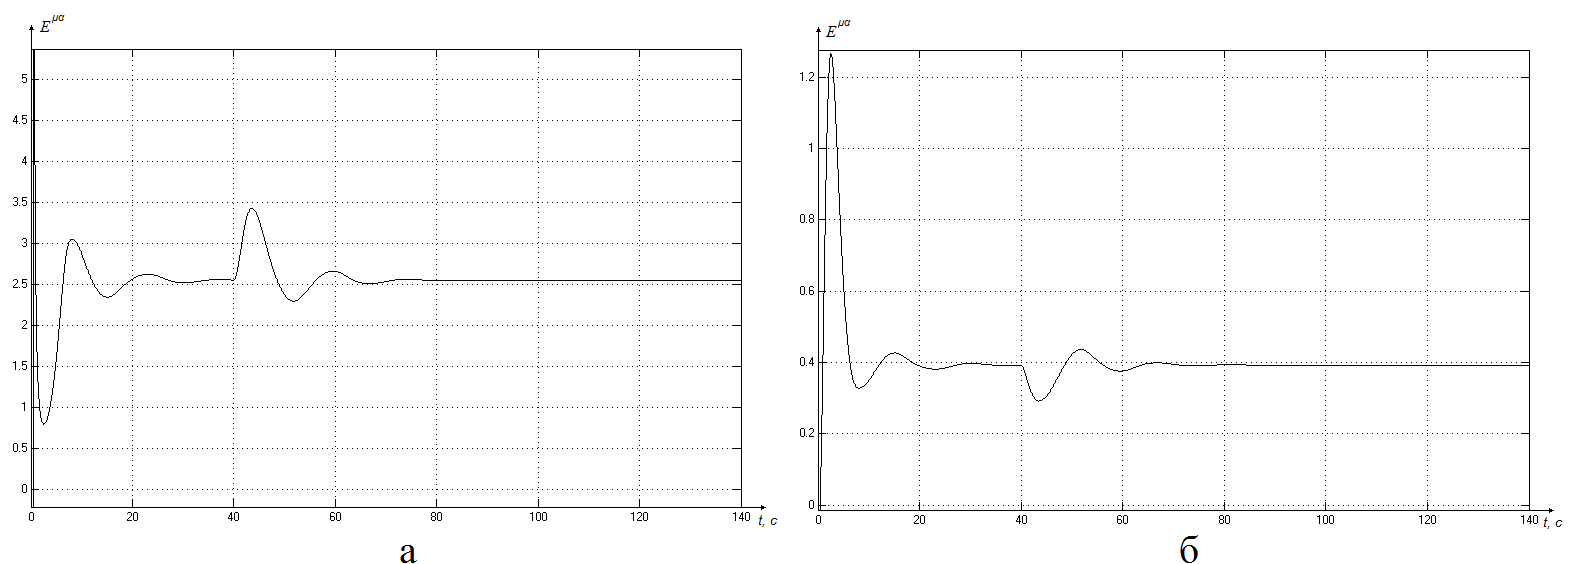
\includegraphics [scale=0.4] {352-4.png}
  \caption{Изменение значений тягового фактора для режима пуска (а) и тягового фактора для режима торможения (б) при весе натяжного устройства, равном $ 65000 H $} 
  \label{img.3.pf}  
\end{figure}

Так как процесс останова конвейера занимает очень малое время по сравнению с временем рабочего режима, то целесообразно выбрать такой вес натяжного устройства, при котором значение тягового фактора для режима пуска и разгона будет удовлетворять условию Эйлера. В этом случае при останове конвейера необходимо решать задачу стабилизации тягового фактора для~режима торможения для избежания проскальзывания ленты. 

\subsection{Останов конвейера с использованием торможения приводного барабана} \label{subsect3_5_3}
При торможении конвейера, в отличие от свободного выбега, необходимо учитывать создаваемый тормозным устройством тормозной момент $ M_T $, приложенный к приводному или хвостовому барабану и направленный в сторону, противоположную движению барабана. Для исследования режимов торможения используется модифицированная модель ленточного конвейера, которая описана в разделе ~\ref{sect3_3}.\\

Рассмотрим останов конвейера с приложением тормозного момента определенной величины ($ 15000 \text{Нм} $) к приводному барабану. Технологически эта операция осуществляется отключением привода и одновременным включением тормозного устройства на приводном барабане. После отключения лента некоторое продолжает движение под действием сил инерции, а за счет наличия тормозного момента это время значительно сокращается. Проведем моделирование торможения конвейера при скорости движения ленты, равной $1,2$ м/с. На рис.~\ref{img.3.brake4} представлены графики переходных процессов по скоростям сосредоточенных масс ленты и натяжного устройства.

\begin{figure} [h] 
  \center
  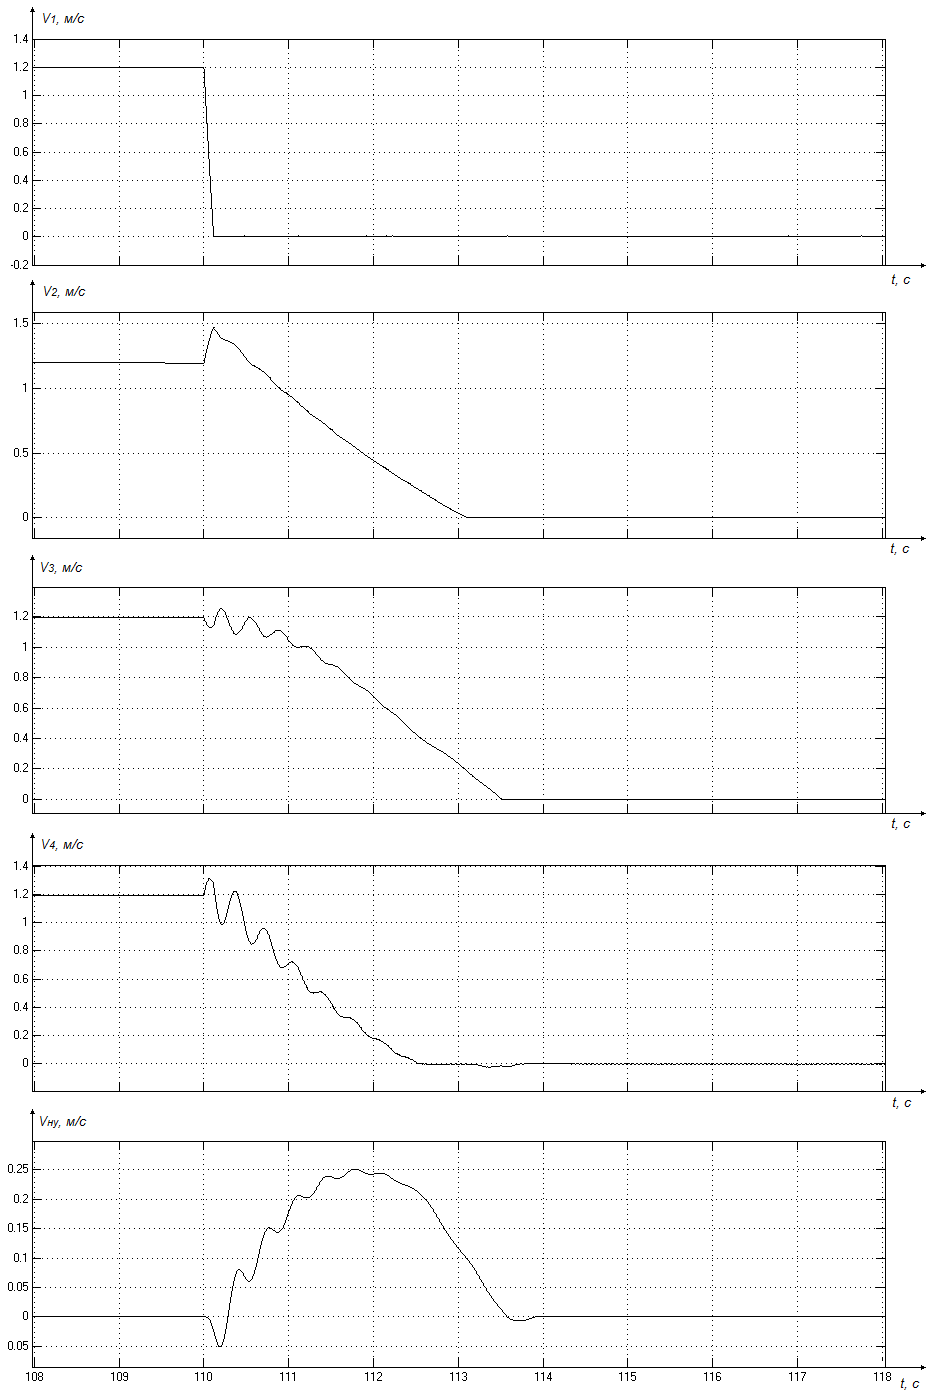
\includegraphics [scale=0.65] {353-1.png}
  \caption{Переходные процессы по скоростям сосредоточенных масс ленты и натяжного устройства при останове конвейера с торможением приводного барабана} 
  \label{img.3.brake4}  
\end{figure}

Из рис.~\ref{img.3.brake4} видно, что приводной барабан (и точка, соответствующая первой сосредоточенной массе ленты) останавливается значительно быстрее, чем при останове конвейера без применения торможения (рис. \ref{img.3.brake1}). Останов приводного барабана в данном случае осуществляется за $ 0,12 $ сек. Останов остальных сосредоточенных масс ленты происходит за $ 3 - 4 $ сек, при этом наблюдается колебательный характер уменьшения скоростей сосредоточенных масс.

На рис.~\ref{img.3.brake5} представлен график изменения натяжений ленты в точках набегания ленты на приводной барабан и сбегания ленты с приводного барабана. В отличие от останова конвейера без применения торможения, в данном случае значения натяжений изменяются с более высокой скоростью, которая, однако, незначительно отличается от скорости изменения натяжений при останове конвейера без применения торможения в следствие упругости ленты.

На рис.~\ref{img.3.brake6} представлен график изменения величины тягового фактора при останове конвейера с торможением приводного барабана. Этот график показывает, что на протяжении всего времени торможения на приводном барабане присутствует проскальзывание ленты, как и в случае останова конвейера без применения торможения.

\begin{figure} [h] 
  \center
  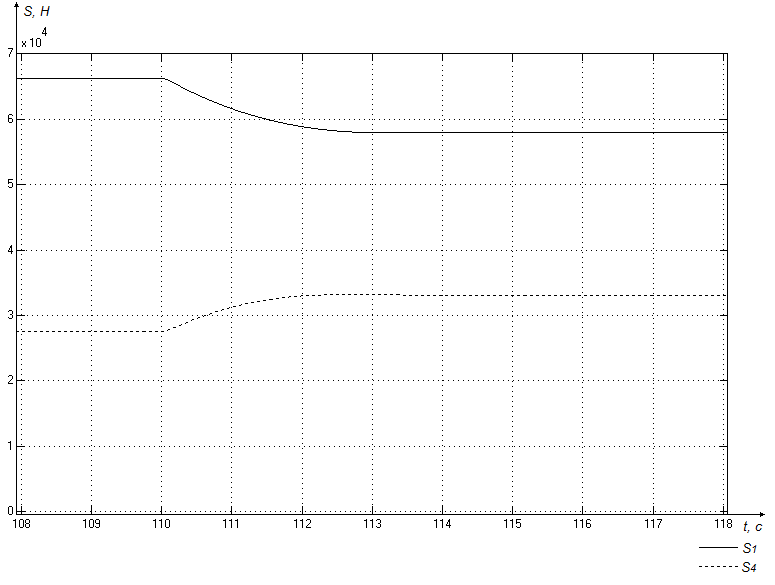
\includegraphics [scale=0.7] {353-2.png}
  \caption{Изменение натяжений в точках набегания ленты на приводной барабан и сбегания ленты с приводного барабана при останове конвейера с торможением приводного барабана} 
  \label{img.3.brake5}  
\end{figure}

\begin{figure} [h] 
  \center
  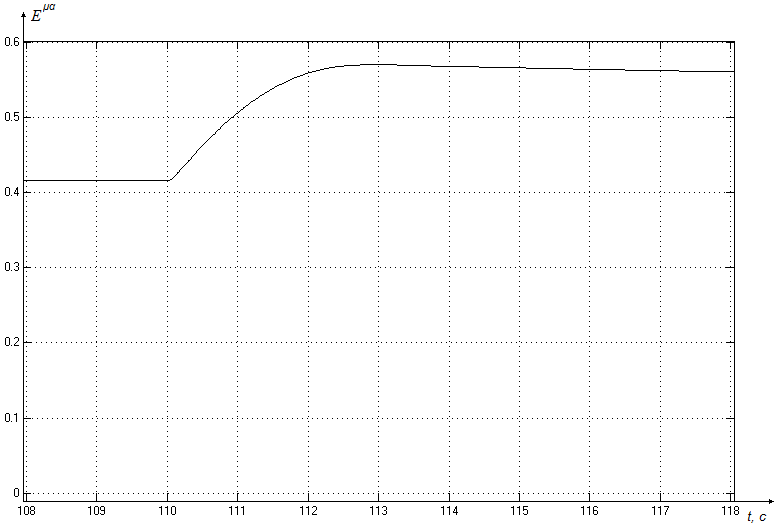
\includegraphics [scale=0.7] {353-3.png}
  \caption{Изменение величины тягового фактора при останове конвейера с торможением приводного барабана} 
  \label{img.3.brake6}  
\end{figure}
\clearpage

\subsection{Торможение хвостового барабана конвейера} \label{subsect3_5_4}
Рассмотрим случай частичного торможения хвостового барабана конвейера без отключения привода (без останова конвейера). Этот случай позволяет наблюдать поведение участков ленты при создании дополнительного тормозного момента на хвостовом барабане и представляет определенный интерес для разработки алгоритма останова конвейера, который обеспечивает контроль проскальзывания ленты.

Рассмотрим торможение хвостового барабана с приложением к нему тормозного момента определенной величины ($ 500 \text{ Нм} $. Технологически эта операция осуществляется включением тормозного устройства на хвостовом барабане в определенное время (привод конвейера при этом не отключается). Проведем моделирование торможения конвейера при скорости движения ленты, равной $1,2$ м/с. Через $ 100 $ секунд после пуска конвейера включим тормозное устройство и еще через $ 60 $ секунд отключим его. На рис.~\ref{img.3.brake7} представлены графики переходных процессов по скоростям сосредоточенных масс ленты и натяжного устройства.

При приложении тормозного момента к хвостовому барабану скорость его движения уменьшается (об этом можно судить по графику скорости сосредоточенной массы $ m_3 $). Через $ 20 $ секунд скорость сосредоточенной массы $ m_3 $ восстанавливается до номинальной величины. При этом на хвостовом барабане, возможно, имеет место проскальзывание ленты. Для контроля проскальзывания ленты на хвостовом барабане необходимо вычислять натяжения ленты в соответствующих точках и величину тягового фактора для хвостового барабана. Величину тормозного момента необходимо выбирать таким образом, чтобы величина тягового фактора не превышала номинального значения. Вычисление натяжений и тягового фактора для случая торможения хвостового барабана описано в разделе \ref{sect3_4}.

При отключении тормозного устройства наблюдается кратковременное увеличение скоростей сосредоточенных масс и последующее восстановление скоростей до номинальной величины.  

Интерес в этом случае представляет изменение значений натяжений в точках набегания ленты на приводной барабан и сбегания ленты с приводного барабана. Как видно из рис.~\ref{img.3.brake8}, при торможении хвостового барабана натяжение в точке набегания ленты на приводной барабан увеличивается на $ 2440 $ Н до величины $ 68700 $ Н, натяжение в точке сбегания ленты с приводного барабана уменьшается на $ 2540 $ Н до величины $ 25000 $ Н. Величина тягового фактора для режима торможения (рис.~\ref{img.3.brake9}), равного отношению натяжения в точке сбегания ленты с приводного барабана к натяжению в точке набегания ленты на приводной барабан, уменьшается и достигает величины $ 0,36 $. Это означает, что в таком режиме (при достаточно низкой величине тягового фактора для режима торможения) может быть произведен останов конвейера (свободным выбегом или с применением торможения приводного барабана) без проскальзывания ленты на приводном барабане.

\begin{figure} [h] 
  \center
  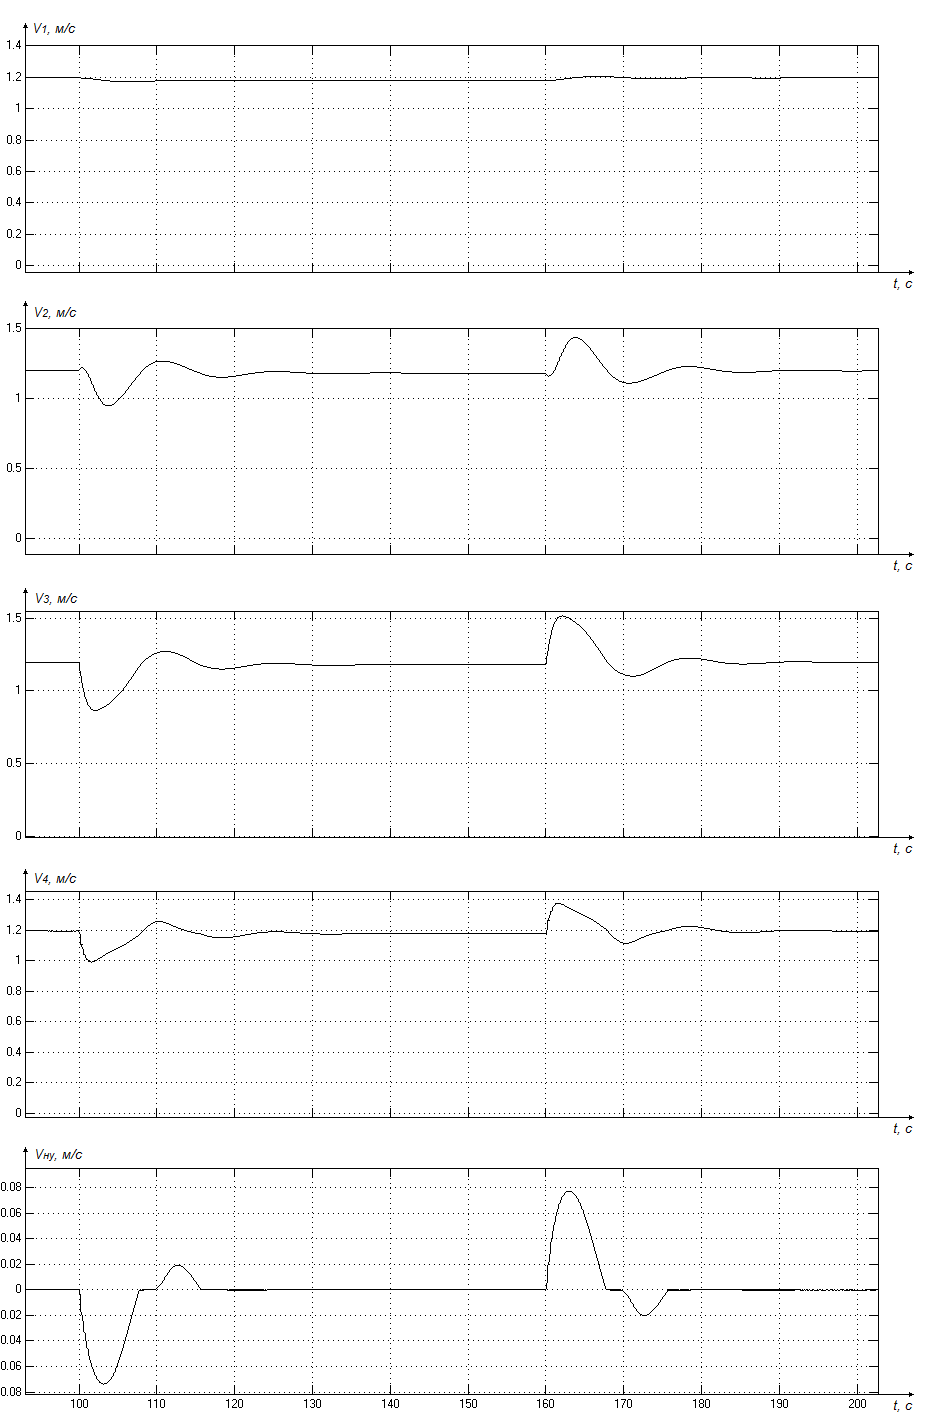
\includegraphics [scale=0.65] {354-1.png}
  \caption{Переходные процессы по скоростям сосредоточенных масс ленты и натяжного устройства при торможении хвостового барабана конвейера} 
  \label{img.3.brake7}  
\end{figure}

\begin{figure} [h] 
  \center
  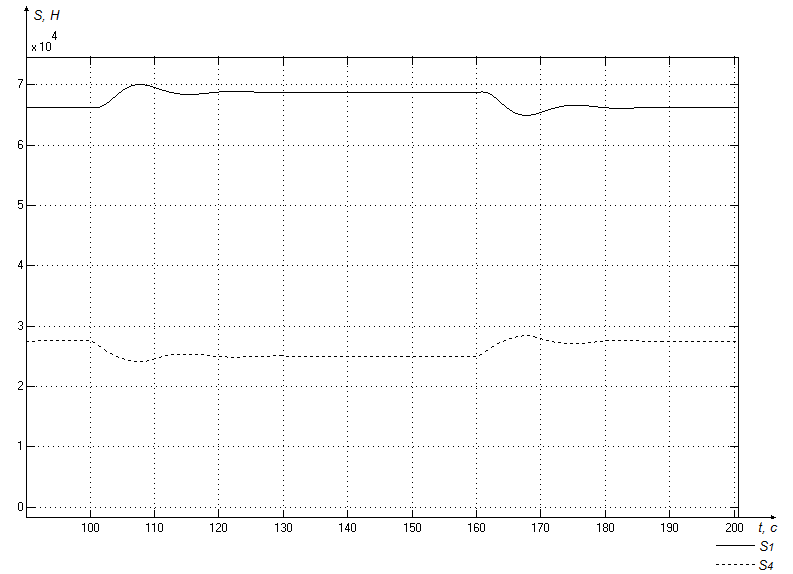
\includegraphics [scale=0.75] {354-2.png}
  \caption{Изменение натяжений в точках набегания ленты на приводной барабан и сбегания ленты с приводного барабана при торможении хвостового барабана конвейера} 
  \label{img.3.brake8}  
\end{figure}

\begin{figure} [h] 
  \center
  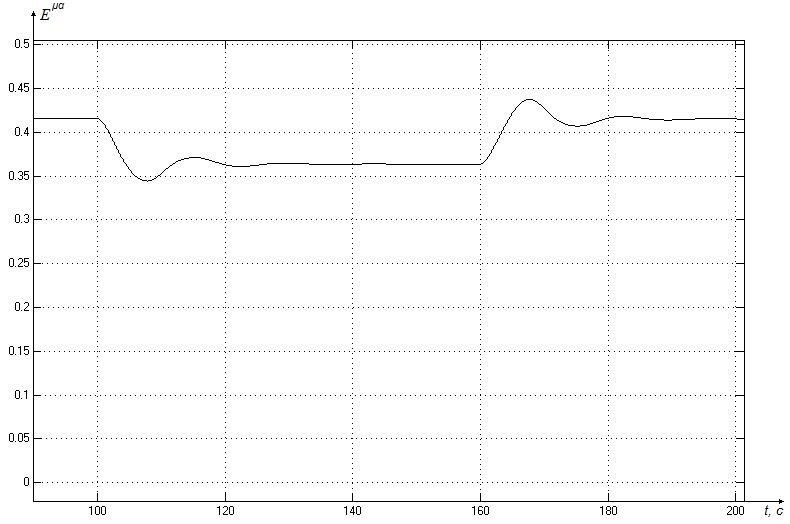
\includegraphics [scale=0.75] {354-3.png}
  \caption{Изменение величины тягового фактора при торможении хвостового барабана конвейера} 
  \label{img.3.brake9}  
\end{figure}
\clearpage

\section{Выводы по главе \ref{chapt3}} \label{subsect3_6}
В настоящей главе описана и модифицирована математическая модель ленточного конвейера, которая вполне соответствует реальному технологическому объекту, а также проведены исследования и анализ параметров следующих переходных процессов конвейерной установки в различных режимах ее работы:
\begin{itemize}
\item Переходные процессы по координатам сосредоточенных масс ленты конвейера и натяжного устройства;
\item Переходные процессы по скоростям сосредоточенных масс ленты конвейера и натяжного устройства;
\item Переходные процессы по изменению натяжений ленты, вычисление которых осуществляется на основе деформаций ленты;
\item Переходные процессы по изменению величины тягового фактора, которые позволяют судить о наличии проскальзывания ленты в определенные периоды времени.
\end{itemize}

Анализ переходных процессов рассмотрен как для режимов пуска и разгона, так и для режима останова (торможения) конвейера. Проведенный анализ позволяет определить набор алгоритмов управления и функций, которые должны входить в состав разрабатываемой комплексной автоматической системы управления конвейером:
\begin{itemize}
\item Алгоритм пуска конвейера и регулирования скорости движения ленты. Этот алгоритм управления должен обеспечивать пуск конвейера с выводом на заданную ползучую скорость, ожидать завершения переходных процессов в ленте и обеспечить переключение на номинальную скорость. Кроме того, алгоритм должен обеспечивать плавное переключение скорости движения ленты с применением оптимального регулятора. Переключение скорости движения ленты должно производиться совместно с работой алгоритма стабилизации тягового фактора конвейера для устранения проскальзывания ленты при переключении скорости ее движения;
\item Алгоритм стабилизации тягового фактора конвейера для устранения проскальзывания ленты в номинальном режиме работы конвейера. Стабилизация тягового фактора осуществляется посредством изменения веса натяжного устройства. Алгоритм стабилизации реализован по традиционной одноконтурной схеме. На вход регулятора натяжения подается сигнал рассогласования $ \varepsilon(t) $ между технологически необходимым значением тягового фактора $ e_0^{\mu \alpha} $, и текущим, вычисляемым значением $ e^{\mu \alpha}(t) $. В зависимости от величины и знака рассогласования должен изменяться вес груза натяжного устройства, либо перемещаться каретка автоматического натяжного устройства. Сигнал об изменении веса груза натяжного устройства или о перемещении каретки автоматического натяжного устройства подается в качестве управляющего сигнала исполнительному механизму, управляющему натяжным устройством конвейера. При этом происходит изменение натяжений $ S_1(t) $ и $ S_4(t) $, и, следовательно, стабилизация величины тягового фактора $ e^{\mu \alpha}(t) $. Подробное описание алгоритма, синтез регулятора и моделирование описаны в~\cite{vdmitrieva};
\item Алгоритм стабилизации тягового фактора конвейера для устранения проскальзывания ленты при останове (торможении) конвейера. Предполагается осуществлять стабилизацию тягового фактора за счет предварительного управляемого торможения хвостового и приводного барабанов конвейера. При торможении хвостового барабана изменяются натяжения $ S_{\text{п}}(t) $ и $ S_{\text{г}}(t) $ в точках набегания ленты на приводной барабан и сбегания ленты с приводного барабана до определенных величин и, соответственно, изменяется величина тягового фактора $ \frac{1}{E^{\mu \alpha}(t)} $ до технологически необходимого значения $ \frac{1}{E_0^{\mu \alpha}} $, что позволяет осуществить снижение скорости, останов или торможение конвейера без проскальзывания ленты на приводном барабане. 

Подробное описание этого алгоритма и особенности его работы представлены в главе~\ref{chapt4}.

\item Контроль провисания ленты конвейера при останове (торможении) конвейера. При снижении скорости движения ленты натяжение в грузовой ветви может уменьшиться до такой величины, при которой будет наблюдаться провисание ленты между роликоопорами. 
Для контроля этого процесса необходимо обеспечивать требуемое технологическое значение натяжения грузовой ветви ленты конвейера после его останова~\cite{vdmitriev}. Это значение рассчитывается по формуле

$$ S_{min} = 5 \div 8(q_\text{г} + q_\text{л})l_p^{'}, $$

где $ q_\text{г}$ и $q_\text{л} $ -- погонный вес грузовой и порожней ветвей соответственно, $ l_p^{'} $ -- расстояние между роликоопорами конвейера.

Подробное описание этого алгоритма и особенности его работы представлены в главе~\ref{chapt4};

\end{itemize}

Проведенный анализ также позволяет сформулировать следующие требования и рекомендации к разрабатываемым алгоритмам в частности и комплексной автоматической системе управления конвейером в общем:

\begin{itemize}
\item Комплексная автоматизированная система управления конвейером должна быть реализована на современном программном и аппаратном обеспечении, рассчитанном на работу в сложных условиях горных предприятий;
\item Комплексная автоматизированная система управления конвейером должна совмещать в себе все описанные алгоритмы управления, быть легко масштабируемой для реализации новых алгоритмов управления и возможности резервирования;
\item Комплексная автоматизированная система управления конвейером должна позволять осуществлять работу нескольких описанных алгоритмов совместно;
\item Комплексная автоматизированная система управления конвейером должна поддерживать свою работу как в номинальном, так и в аварийном (экстренное торможение) режимах работы конвейера;
\item Комплексная автоматизированная система управления конвейером должна предусматривать возможность отключения для обеспечения ручного режима управления конвейером;
\item Алгоритм стабилизации тягового фактора конвейера для устранения проскальзывания ленты при переключении скорости с меньшей на большую должен использоваться при пуске конвейера и увеличении скорости движения ленты только в случаях возможного возникновения проскальзывания ленты. Случаи возможного возникновения проскальзывания ленты определяются на основе текущего значения тягового фактора $ E^{\mu \alpha}(t) $.
\item Алгоритм стабилизации тягового фактора конвейера для устранения проскальзывания ленты при останове конвейера должен также использоваться только в случаях возможного возникновения проскальзывания ленты. Случаи возможного возникновения проскальзывания ленты определяются на основе текущего значения тягового фактора $ \frac{1}{E^{\mu \alpha}(t)} $.
\end{itemize}